% =============================================================================
%  AIAA Region II Student Conference 2026 -- Group Presentation
%  University of South Carolina -- Maritime Perception Lab
% =============================================================================
\documentclass[aspectratio=169, 10pt]{beamer}

% --- Packages ----------------------------------------------------------------
\usepackage[T1]{fontenc}
\usepackage{lmodern}
\usepackage{graphicx}
\usepackage{booktabs}
\usepackage{amsmath,amssymb}
\usepackage{tikz}
\usetikzlibrary{arrows.meta, positioning, shapes.geometric, fit, calc, backgrounds}
\usepackage{pgfplots}
\pgfplotsset{compat=1.18}
\usepackage{array}
\usepackage{colortbl}
\usepackage{multicol}
\usepackage{ragged2e}
\usepackage{caption}
\captionsetup{font=scriptsize, labelformat=empty}

% --- Brand Colors ------------------------------------------------------------
\definecolor{Garnet}{HTML}{73000A}
\definecolor{GarnetDark}{HTML}{500007}
\definecolor{Rose}{HTML}{CC2E40}
\definecolor{Atlantic}{HTML}{466A9F}
\definecolor{Congaree}{HTML}{1F414D}
\definecolor{Horseshoe}{HTML}{65780B}
\definecolor{Grass}{HTML}{CED318}
\definecolor{Honeycomb}{HTML}{A49137}
\definecolor{WarmGrey}{HTML}{676156}
\definecolor{Sandstorm}{HTML}{FFF2E3}
\definecolor{Black90}{HTML}{363636}
\definecolor{Black70}{HTML}{5C5C5C}
\definecolor{Black50}{HTML}{A2A2A2}
\definecolor{Black30}{HTML}{C7C7C7}
\definecolor{Black10}{HTML}{ECECEC}

% --- Beamer Theme (Minimal, Sharp Edges) -------------------------------------
\usetheme{default}
\useinnertheme{default}
\useoutertheme{default}

% Remove all rounded corners
\setbeamertemplate{blocks}[default]
\setbeamertemplate{title page}[default]
\setbeamertemplate{itemize items}[square]
\setbeamertemplate{enumerate items}[default]

% Color assignments
\setbeamercolor{structure}{fg=Garnet}
\setbeamercolor{palette primary}{bg=Garnet, fg=white}
\setbeamercolor{palette secondary}{bg=Congaree, fg=white}
\setbeamercolor{palette tertiary}{bg=Atlantic, fg=white}
\setbeamercolor{frametitle}{bg=Garnet, fg=white}
\setbeamercolor{title}{fg=white, bg=Garnet}
\setbeamercolor{subtitle}{fg=Black30}
\setbeamercolor{author}{fg=Black90}
\setbeamercolor{date}{fg=Black70}
\setbeamercolor{institute}{fg=Black70}
\setbeamercolor{block title}{bg=Garnet, fg=white}
\setbeamercolor{block body}{bg=Black10, fg=Black90}
\setbeamercolor{block title alerted}{bg=Rose, fg=white}
\setbeamercolor{block body alerted}{bg=Black10, fg=Black90}
\setbeamercolor{block title example}{bg=Congaree, fg=white}
\setbeamercolor{block body example}{bg=Black10, fg=Black90}
\setbeamercolor{item}{fg=Garnet}
\setbeamercolor{section in toc}{fg=Black90}
\setbeamercolor{normal text}{fg=Black90}
\setbeamercolor{footline}{bg=Black90, fg=white}

% Font assignments
\setbeamerfont{frametitle}{size=\large, series=\bfseries}
\setbeamerfont{title}{size=\Large, series=\bfseries}
\setbeamerfont{subtitle}{size=\normalsize}
\setbeamerfont{block title}{size=\normalsize, series=\bfseries}

% Frame title template (sharp rectangle)
\setbeamertemplate{frametitle}{%
  \nointerlineskip
  \begin{beamercolorbox}[wd=\paperwidth, ht=2.5em, dp=0.8em, leftskip=0.5em]{frametitle}%
    \usebeamerfont{frametitle}\insertframetitle%
  \end{beamercolorbox}%
}

% Footline with slide number
\setbeamertemplate{footline}{%
  \begin{beamercolorbox}[wd=\paperwidth, ht=2ex, dp=1ex, leftskip=1em, rightskip=1em]{footline}%
    \scriptsize AIAA Region II Student Conference 2026 \hfill University of South Carolina \hfill \insertframenumber/\inserttotalframenumber%
  \end{beamercolorbox}%
}

\setbeamertemplate{navigation symbols}{}

\tikzset{
  pipebox/.style={rectangle, draw=#1, fill=#1!10, line width=1pt,
                   minimum width=5.5cm, minimum height=0.8cm,
                   font=\small\bfseries, text=#1!80!black, align=center},
  modebox/.style={rectangle, draw=#1, fill=#1!8, line width=0.8pt,
                   minimum width=4.8cm, minimum height=1.1cm,
                   font=\scriptsize, align=center, text=Black90},
  summbox/.style={rectangle, draw=#1, fill=#1!10, line width=1pt,
                   minimum width=6.5cm, minimum height=0.8cm,
                   font=\small, text=Black90, align=left},
}

% --- Macros ------------------------------------------------------------------
\def\sectionframe#1#2{%
  \def\temptitlea{#1}%
  \def\temptitleb{#2}%
  \begin{frame}[plain]
    \begin{tikzpicture}[remember picture, overlay]
      \fill[Garnet] (current page.south west) rectangle (current page.north east);
      \node[anchor=center, text=white, font=\Huge\bfseries, text width=14cm, align=center]
        at ([yshift=0.5cm]current page.center) {\temptitlea};
      \node[anchor=center, text=Black30, font=\large, text width=14cm, align=center]
        at ([yshift=-1.2cm]current page.center) {\temptitleb};
    \end{tikzpicture}
  \end{frame}
}

% =============================================================================
\title{Edge-Deployed Maritime Perception\\for Unmanned Surface Vehicles}
\subtitle{AIAA Region II Student Conference 2026}
\author{%
  J.C.~Vaught \and N.~Kirk \and S.~Cancilla \and J.~Wang\\[0.3em]
  \textit{Advisors:} D.~Cahl, Y.~Wang%
}
\institute{Department of Mechanical Engineering\\University of South Carolina}
\date{2026}

\begin{document}

% =============================================================================
% TITLE
% =============================================================================
\begin{frame}[plain]
  \begin{tikzpicture}[remember picture, overlay]
    % Background
    \fill[Garnet] (current page.south west) rectangle (current page.north east);
    % Accent bar
    \fill[GarnetDark] ([yshift=3.5cm]current page.south west) rectangle ([yshift=3.8cm]current page.south east);
    % Title
    \node[anchor=south, text=white, font=\LARGE\bfseries, text width=14cm, align=center]
      at ([yshift=5.0cm]current page.south) {Edge-Deployed Maritime Perception\\for Unmanned Surface Vehicles};
    % Subtitle
    \node[anchor=south, text=Black30, font=\large, text width=14cm, align=center]
      at ([yshift=4.2cm]current page.south) {AIAA Region II Student Conference 2026};
    % Authors
    \node[anchor=north, text=white, font=\normalsize, text width=14cm, align=center]
      at ([yshift=3.2cm]current page.south) {%
        J.C.~Vaught \quad N.~Kirk \quad S.~Cancilla \quad J.~Wang\\[0.3em]
        {\small\textit{Advisors:} D.~Cahl \enspace \& \enspace Y.~Wang}\\[0.3em]
        {\small Department of Mechanical Engineering, University of South Carolina}%
      };
    % Bottom bar
    \node[anchor=south, text=Black50, font=\scriptsize]
      at ([yshift=0.4cm]current page.south) {Columbia, SC \enspace $\cdot$ \enspace 2026};
  \end{tikzpicture}
\end{frame}

% =============================================================================
% OUTLINE
% =============================================================================
\begin{frame}{Overview}
  \begin{columns}[T]
    \begin{column}{0.55\textwidth}
      Four papers addressing the full \textbf{perception pipeline} for autonomous surface vessels using COTS sensors and edge hardware:
      \vspace{0.5em}
      \begin{enumerate}
        \item[\textcolor{Garnet}{\textbf{1}}] \textbf{Synthetic Radar Data} \hfill {\scriptsize Vaught}\\
              {\small Multi-mode simulation for training data generation}
        \vspace{0.4em}
        \item[\textcolor{Atlantic}{\textbf{2}}] \textbf{CFAR Autotuning} \hfill {\scriptsize Kirk}\\
              {\small Human-supervised detection parameter optimization}
        \vspace{0.4em}
        \item[\textcolor{Congaree}{\textbf{3}}] \textbf{Adaptive ST-DBSCAN} \hfill {\scriptsize Cancilla}\\
              {\small Real-time clustering and multi-sweep tracking}
        \vspace{0.4em}
        \item[\textcolor{Horseshoe}{\textbf{4}}] \textbf{Dual-Camera Acquisition} \hfill {\scriptsize Wang}\\
              {\small Active optical verification and auto-labeling}
      \end{enumerate}
    \end{column}
    \begin{column}{0.42\textwidth}
      \centering
      % Pipeline flow diagram
      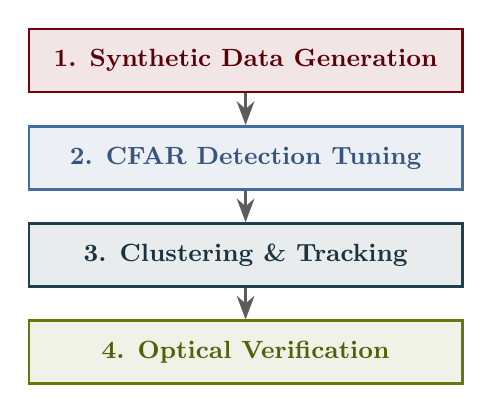
\begin{tikzpicture}[
        arr/.style={-{Stealth[length=3mm]}, thick, color=Black70},
        node distance=0.4cm
      ]
        \node[pipebox=Garnet] (s1) {1. Synthetic Data Generation};
        \node[pipebox=Atlantic, below=of s1] (s2) {2. CFAR Detection Tuning};
        \node[pipebox=Congaree, below=of s2] (s3) {3. Clustering \& Tracking};
        \node[pipebox=Horseshoe, below=of s3] (s4) {4. Optical Verification};
        \draw[arr] (s1) -- (s2);
        \draw[arr] (s2) -- (s3);
        \draw[arr] (s3) -- (s4);
      \end{tikzpicture}
    \end{column}
  \end{columns}
\end{frame}

% =============================================================================
% SHARED PLATFORM
% =============================================================================
\begin{frame}{Shared Sensor Platform \& Field Sites}
  \begin{columns}[T]
    \begin{column}{0.48\textwidth}
      \begin{block}{Common Hardware}
        {\small
        \begin{itemize}\setlength{\itemsep}{0pt}
          \item \textbf{Radar:} Furuno DRS4D NXT X-band
            \begin{itemize}
              \item[$\circ$] 9.38--9.44\,GHz, solid-state, 100\,W
              \item[$\circ$] LFM chirp, $\sim$20\,m range resolution
              \item[$\circ$] 3.9$^\circ$ beamwidth, 24/36/48 RPM
            \end{itemize}
          \item \textbf{Cameras:} 2$\times$ FLIR M300C (wide + PTZ)
          \item \textbf{Edge compute:}
            \begin{itemize}
              \item[$\circ$] NVIDIA Jetson AGX Orin (32\,GB)
              \item[$\circ$] Raspberry Pi 5 (browser-based tools)
            \end{itemize}
          \item \textbf{Battery:} 12.8\,V / 50\,Ah LiFePO$_4$
        \end{itemize}
        }
      \end{block}
    \end{column}
    \begin{column}{0.48\textwidth}
      \begin{block}{Field Collection Sites (South Carolina)}
        {\small
        \begin{itemize}\setlength{\itemsep}{0pt}
          \item Lake Murray -- primary test site
          \item Lake Greenwood -- inland variety
          \item Charleston Harbor -- coastal/maritime
        \end{itemize}
        \vspace{0.2em}
        $\sim$30 sessions over 11 months\\
        Targets: recreational boats, pontoons, buoys
        }
      \end{block}
      \vspace{0.2em}
      \begin{block}{Target Characteristics}
        {\small
        \begin{itemize}\setlength{\itemsep}{0pt}
          \item Fiberglass boats: $\sigma = 0.5$--$20\,\text{m}^2$
          \item Aluminum / buoys: $\sigma = 1$--$50\,\text{m}^2$
          \item Antenna height: 2--4\,m above water
          \item Grazing angle: $\approx 0.19^\circ$ at 500\,m
        \end{itemize}
        }
      \end{block}
    \end{column}
  \end{columns}
\end{frame}

% =============================================================================
% PAPER 1 -- VAUGHT: SYNTHETIC RADAR
% =============================================================================
\begin{frame}[plain]
  \begin{tikzpicture}[remember picture, overlay]
    \fill[Garnet] (current page.south west) rectangle (current page.north east);
    \node[anchor=center, text=white, font=\Huge\bfseries, text width=14cm, align=center]
      at ([yshift=0.5cm]current page.center) {Paper 1};
    \node[anchor=center, text=Black30, font=\large, text width=14cm, align=center]
      at ([yshift=-1.2cm]current page.center) {A Multi-Mode Simulation Framework\\for X-Band Pulse Compression Radar\\[0.3em]\normalsize J.C. Vaught, D. Cahl, Y. Wang};
  \end{tikzpicture}
\end{frame}

% --- Motivation ---
\begin{frame}{Synthetic Radar -- Motivation}
  \begin{columns}[T]
    \begin{column}{0.55\textwidth}
      \begin{block}{The Problem}
        {\small
        \begin{itemize}\setlength{\itemsep}{1pt}
          \item Maritime radar data is \textbf{scarce} and expensive
          \item Manual labeling of radar returns is ambiguous
          \item Coverage of rare events is limited
          \item Domain shift between environments
        \end{itemize}
        }
      \end{block}
      \vspace{0.15em}
      \begin{block}{Three-Mode Synthetic Framework}
        {\small
        \begin{itemize}\setlength{\itemsep}{1pt}
          \item \textbf{Mode 1:} Data-driven compositing (fast)
          \item \textbf{Mode 2:} Analytical clutter generation
          \item \textbf{Mode 3:} EM ray tracing (physics valid.)
        \end{itemize}
        }
      \end{block}
    \end{column}
    \begin{column}{0.42\textwidth}
      \centering
      % Architecture diagram
      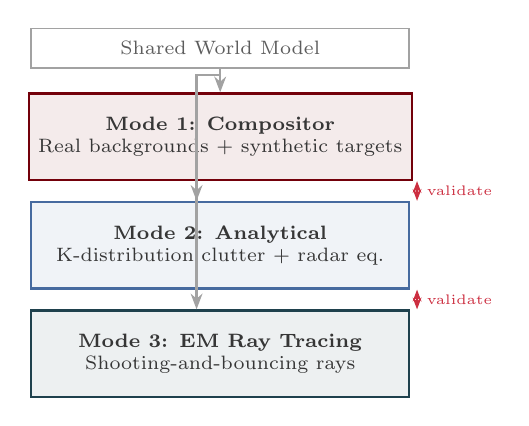
\begin{tikzpicture}[
        wbox/.style={rectangle, draw=Black50, fill=white, line width=0.6pt,
                      minimum width=4.8cm, minimum height=0.5cm,
                      font=\scriptsize, align=center, text=Black70},
        arr/.style={-{Stealth[length=2mm]}, thick, color=Black50},
        node distance=0.25cm
      ]
        \node[wbox] (world) {Shared World Model};
        \node[modebox=Garnet, below=0.3cm of world] (m1)
          {\textbf{Mode 1: Compositor}\\Real backgrounds + synthetic targets};
        \node[modebox=Atlantic, below=of m1] (m2)
          {\textbf{Mode 2: Analytical}\\K-distribution clutter + radar eq.};
        \node[modebox=Congaree, below=of m2] (m3)
          {\textbf{Mode 3: EM Ray Tracing}\\Shooting-and-bouncing rays};
        \draw[arr] (world) -- (m1);
        \draw[arr] (world.south) -- ++(0,-0.08) -| ([xshift=-0.3cm]m2.north);
        \draw[arr] (world.south) -- ++(0,-0.08) -| ([xshift=-0.3cm]m3.north);
        % Cross-validation arrows
        \draw[{Stealth[length=1.5mm]}-{Stealth[length=1.5mm]}, dashed, Rose]
          ([xshift=2.5cm]m1.south) -- ([xshift=2.5cm]m2.north)
          node[midway, right, font=\tiny, text=Rose] {validate};
        \draw[{Stealth[length=1.5mm]}-{Stealth[length=1.5mm]}, dashed, Rose]
          ([xshift=2.5cm]m2.south) -- ([xshift=2.5cm]m3.north)
          node[midway, right, font=\tiny, text=Rose] {validate};
      \end{tikzpicture}
    \end{column}
  \end{columns}
\end{frame}

% --- Three Modes Detail ---
\begin{frame}{Synthetic Radar -- Framework Details}
  \begin{columns}[T]
    \begin{column}{0.32\textwidth}
      \begin{block}{\scriptsize\textcolor{Garnet}{Mode 1: Compositor}}
        {\scriptsize
        \begin{enumerate}\setlength{\itemsep}{0pt}
          \item Background selection
          \item Target signature generation
          \item Amplitude matching
          \item Insertion \& blending
          \item Automatic label generation
        \end{enumerate}
        \vspace{0.2em}
        \textbf{Augmentation:} Real radar interference and rain clutter overlays}
      \end{block}
    \end{column}
    \begin{column}{0.32\textwidth}
      \begin{block}{\scriptsize\textcolor{Atlantic}{Mode 2: Analytical}}
        {\scriptsize K-distribution clutter PDF:}
        \vspace{-0.2em}
        \[
          \scriptstyle f(x) = \frac{2}{\Gamma(\nu)} \left(\frac{\nu}{P_c}\right)^{\frac{\nu+1}{2}} x^\nu K_{\nu-1}\left(2\sqrt{\frac{\nu x}{P_c}}\right)
        \]
        \vspace{-0.6em}
        {\scriptsize
        \begin{itemize}\setlength{\itemsep}{0pt}
          \item Shape $\nu$ controls tail weight
          \item Swerling-I target model
          \item Full B-scan via radar equation
        \end{itemize}
        }
      \end{block}
    \end{column}
    \begin{column}{0.32\textwidth}
      \begin{block}{\scriptsize\textcolor{Congaree}{Mode 3: Ray Tracing}}
        {\scriptsize
        \begin{itemize}\setlength{\itemsep}{0pt}
          \item Shooting-and-bouncing rays
          \item Time-varying water mesh from wave spectrum
          \item Physics validation of Modes 1--2
          \item Shoreline geometry (ongoing)
        \end{itemize}
        }
        \vspace{0.1em}
        {\scriptsize\textbf{Radar Eq:}}
        \vspace{-0.3em}
        \[
          P_r = \frac{P_t G^2 \lambda^2 \sigma}{(4\pi)^3 R^4 L}
        \]
      \end{block}
    \end{column}
  \end{columns}
  \vspace{0.2em}
  \centering
  {\footnotesize\textbf{Domain Transfer:} YOLO detector trained on Mode~1 composites, evaluated on real radar frames}
\end{frame}

% --- Radar Specs Table ---
\begin{frame}{Synthetic Radar -- Sensor Characterization}
  \begin{columns}[T]
    \begin{column}{0.45\textwidth}
      \begin{block}{Furuno DRS4D NXT Specifications}
        \centering
        \small
        \renewcommand{\arraystretch}{1.15}
        \begin{tabular}{@{}l l@{}}
          \toprule
          \textbf{Parameter} & \textbf{Value} \\
          \midrule
          Transmitter     & Solid-state \\
          Frequency        & 9.38--9.44\,GHz \\
          Output Power     & 100\,W \\
          Modulation       & LFM chirp \\
          Pulse Width      & 5--18\,$\mu$s \\
          Range Res.       & $\sim$20\,m \\
          Beamwidth        & 3.9$^\circ$ \\
          Rotation         & 24/36/48\,RPM \\
          PRF              & 700--1100\,Hz \\
          Azimuth Quant.   & 8192 spokes/rev \\
          Radome Dia.      & 610\,mm \\
          \bottomrule
        \end{tabular}
      \end{block}
    \end{column}
    \begin{column}{0.52\textwidth}
      \begin{block}{Data Acquisition}
        \begin{itemize}
          \item UDP multicast capture at spoke rate
          \item B-scan format: range $\times$ azimuth
          \item 30+ collection sessions, 3 SC sites
          \item 11-month campaign
        \end{itemize}
      \end{block}
      \vspace{0.3em}
      \begin{block}{Key Contributions}
        \begin{enumerate}
          \item Multi-mode framework with cross-validation
          \item Sim-to-real domain transfer demonstration
          \item Environmental augmentation strategy
          \item First DRS4D NXT characterization for DL
        \end{enumerate}
      \end{block}
    \end{column}
  \end{columns}
\end{frame}

% =============================================================================
% PAPER 2 -- KIRK: CFAR AUTOTUNING
% =============================================================================
\begin{frame}[plain]
  \begin{tikzpicture}[remember picture, overlay]
    \fill[Garnet] (current page.south west) rectangle (current page.north east);
    \node[anchor=center, text=white, font=\Huge\bfseries, text width=14cm, align=center]
      at ([yshift=0.5cm]current page.center) {Paper 2};
    \node[anchor=center, text=Black30, font=\large, text width=14cm, align=center]
      at ([yshift=-1.2cm]current page.center) {Human-Supervised CFAR Autotuning\\for Maritime Sensing\\[0.3em]\normalsize N. Kirk, J.C. Vaught, D. Cahl, Y. Wang};
  \end{tikzpicture}
\end{frame}

% --- Motivation + UI ---
\begin{frame}{CFAR Autotuning -- CFAR Studio}
  \begin{columns}[T]
    \begin{column}{0.45\textwidth}
      \begin{block}{The Problem}
        {\scriptsize
        \begin{itemize}\setlength{\itemsep}{0pt}\setlength{\topsep}{0pt}
          \item CFAR detectors need tuning: guard cells ($N_g$), reference cells ($N_r$), $P_{FA}$
          \item Heavy-tailed clutter invalidates Gaussian assumptions
          \item Manual tuning is slow and not reproducible
        \end{itemize}
        }
      \end{block}
      \vspace{-0.1em}
      \begin{block}{CFAR Studio -- Open-Source Tool}
        {\scriptsize
        \begin{itemize}\setlength{\itemsep}{0pt}\setlength{\topsep}{0pt}
          \item React 19 + TypeScript, fully client-side
          \item Grid search via Web Worker
          \item Integral images: $O(1)$ noise estimation
          \item \textbf{$\sim$500 configs in $<$10\,seconds}
        \end{itemize}
        }
      \end{block}
    \end{column}
    \begin{column}{0.52\textwidth}
      \centering
      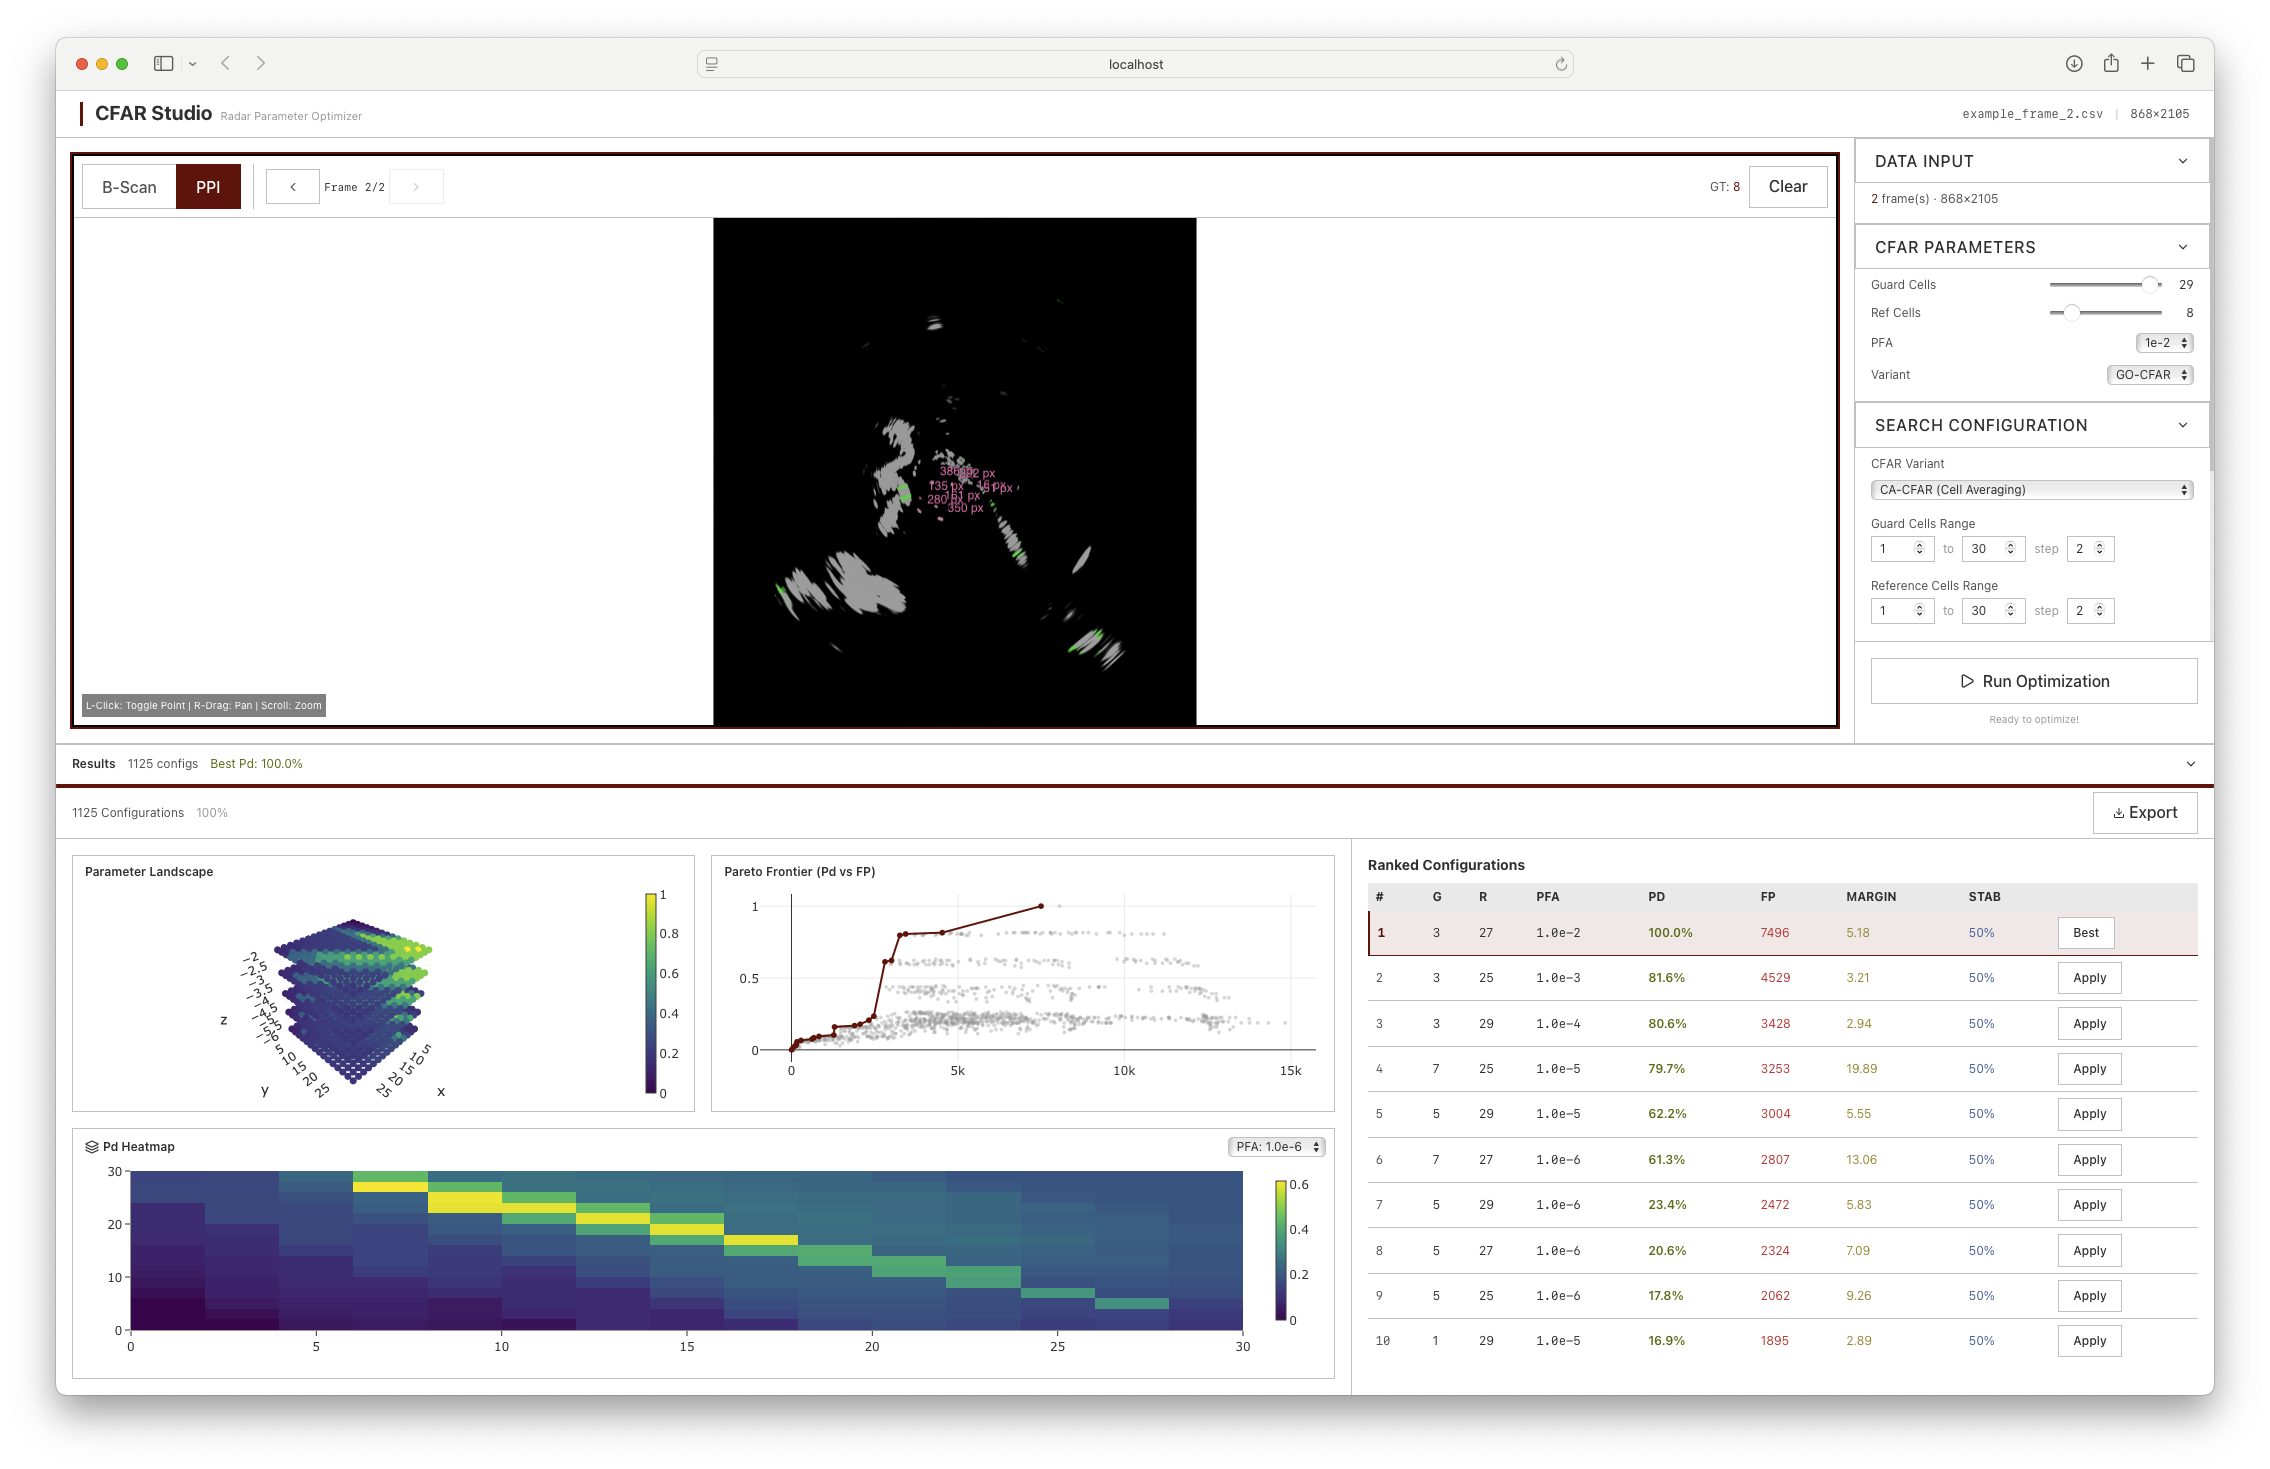
\includegraphics[width=0.95\textwidth, height=0.65\textheight, keepaspectratio]{Kirk_CFAR_Autotuning/figures/full_ui_ppi_with_optimization_results.png}
      \vspace{-0.3em}
      {\scriptsize CFAR Studio: PPI with optimization results dashboard}
    \end{column}
  \end{columns}
\end{frame}

% --- Detection Results ---
\begin{frame}{CFAR Autotuning -- Detection \& Scoring}
  \begin{columns}[T]
    \begin{column}{0.45\textwidth}
      \centering
      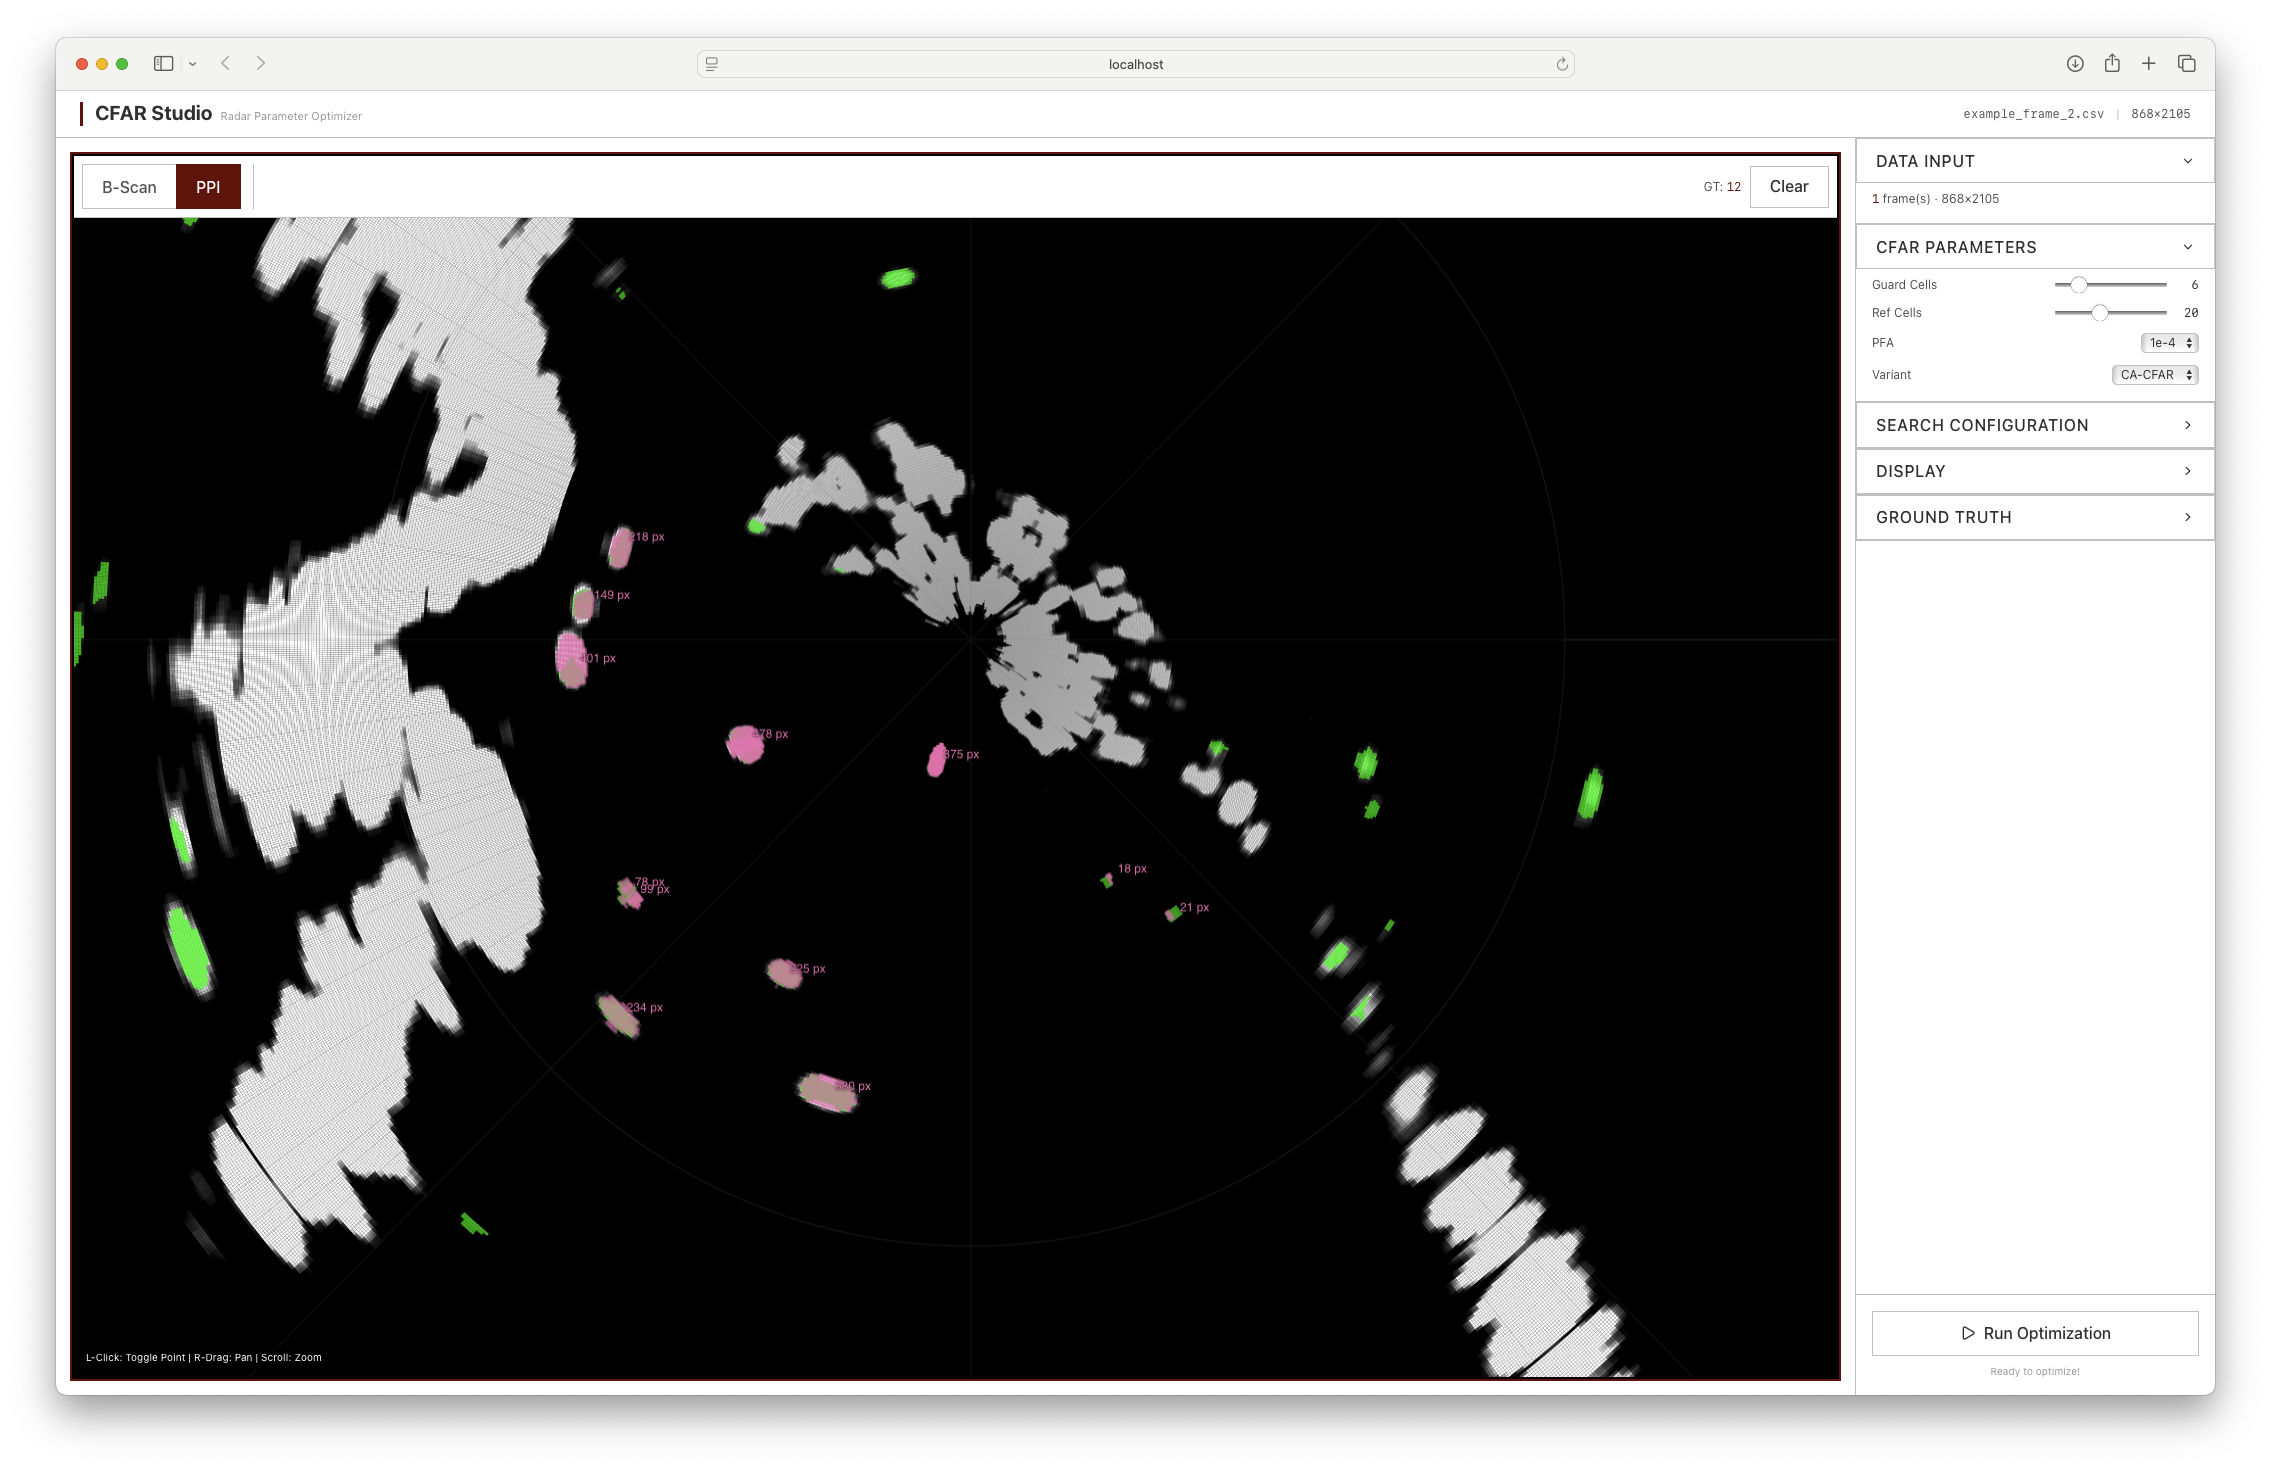
\includegraphics[width=0.95\textwidth, height=2.6cm, keepaspectratio]{Kirk_CFAR_Autotuning/figures/ppi_full_view_detections_and_ground_truth.png}
      \vspace{-0.3em}
      {\scriptsize PPI: CFAR detections {\color{green!70!black}(green)} vs.\ ground truth {\color{Rose}(pink)}}

      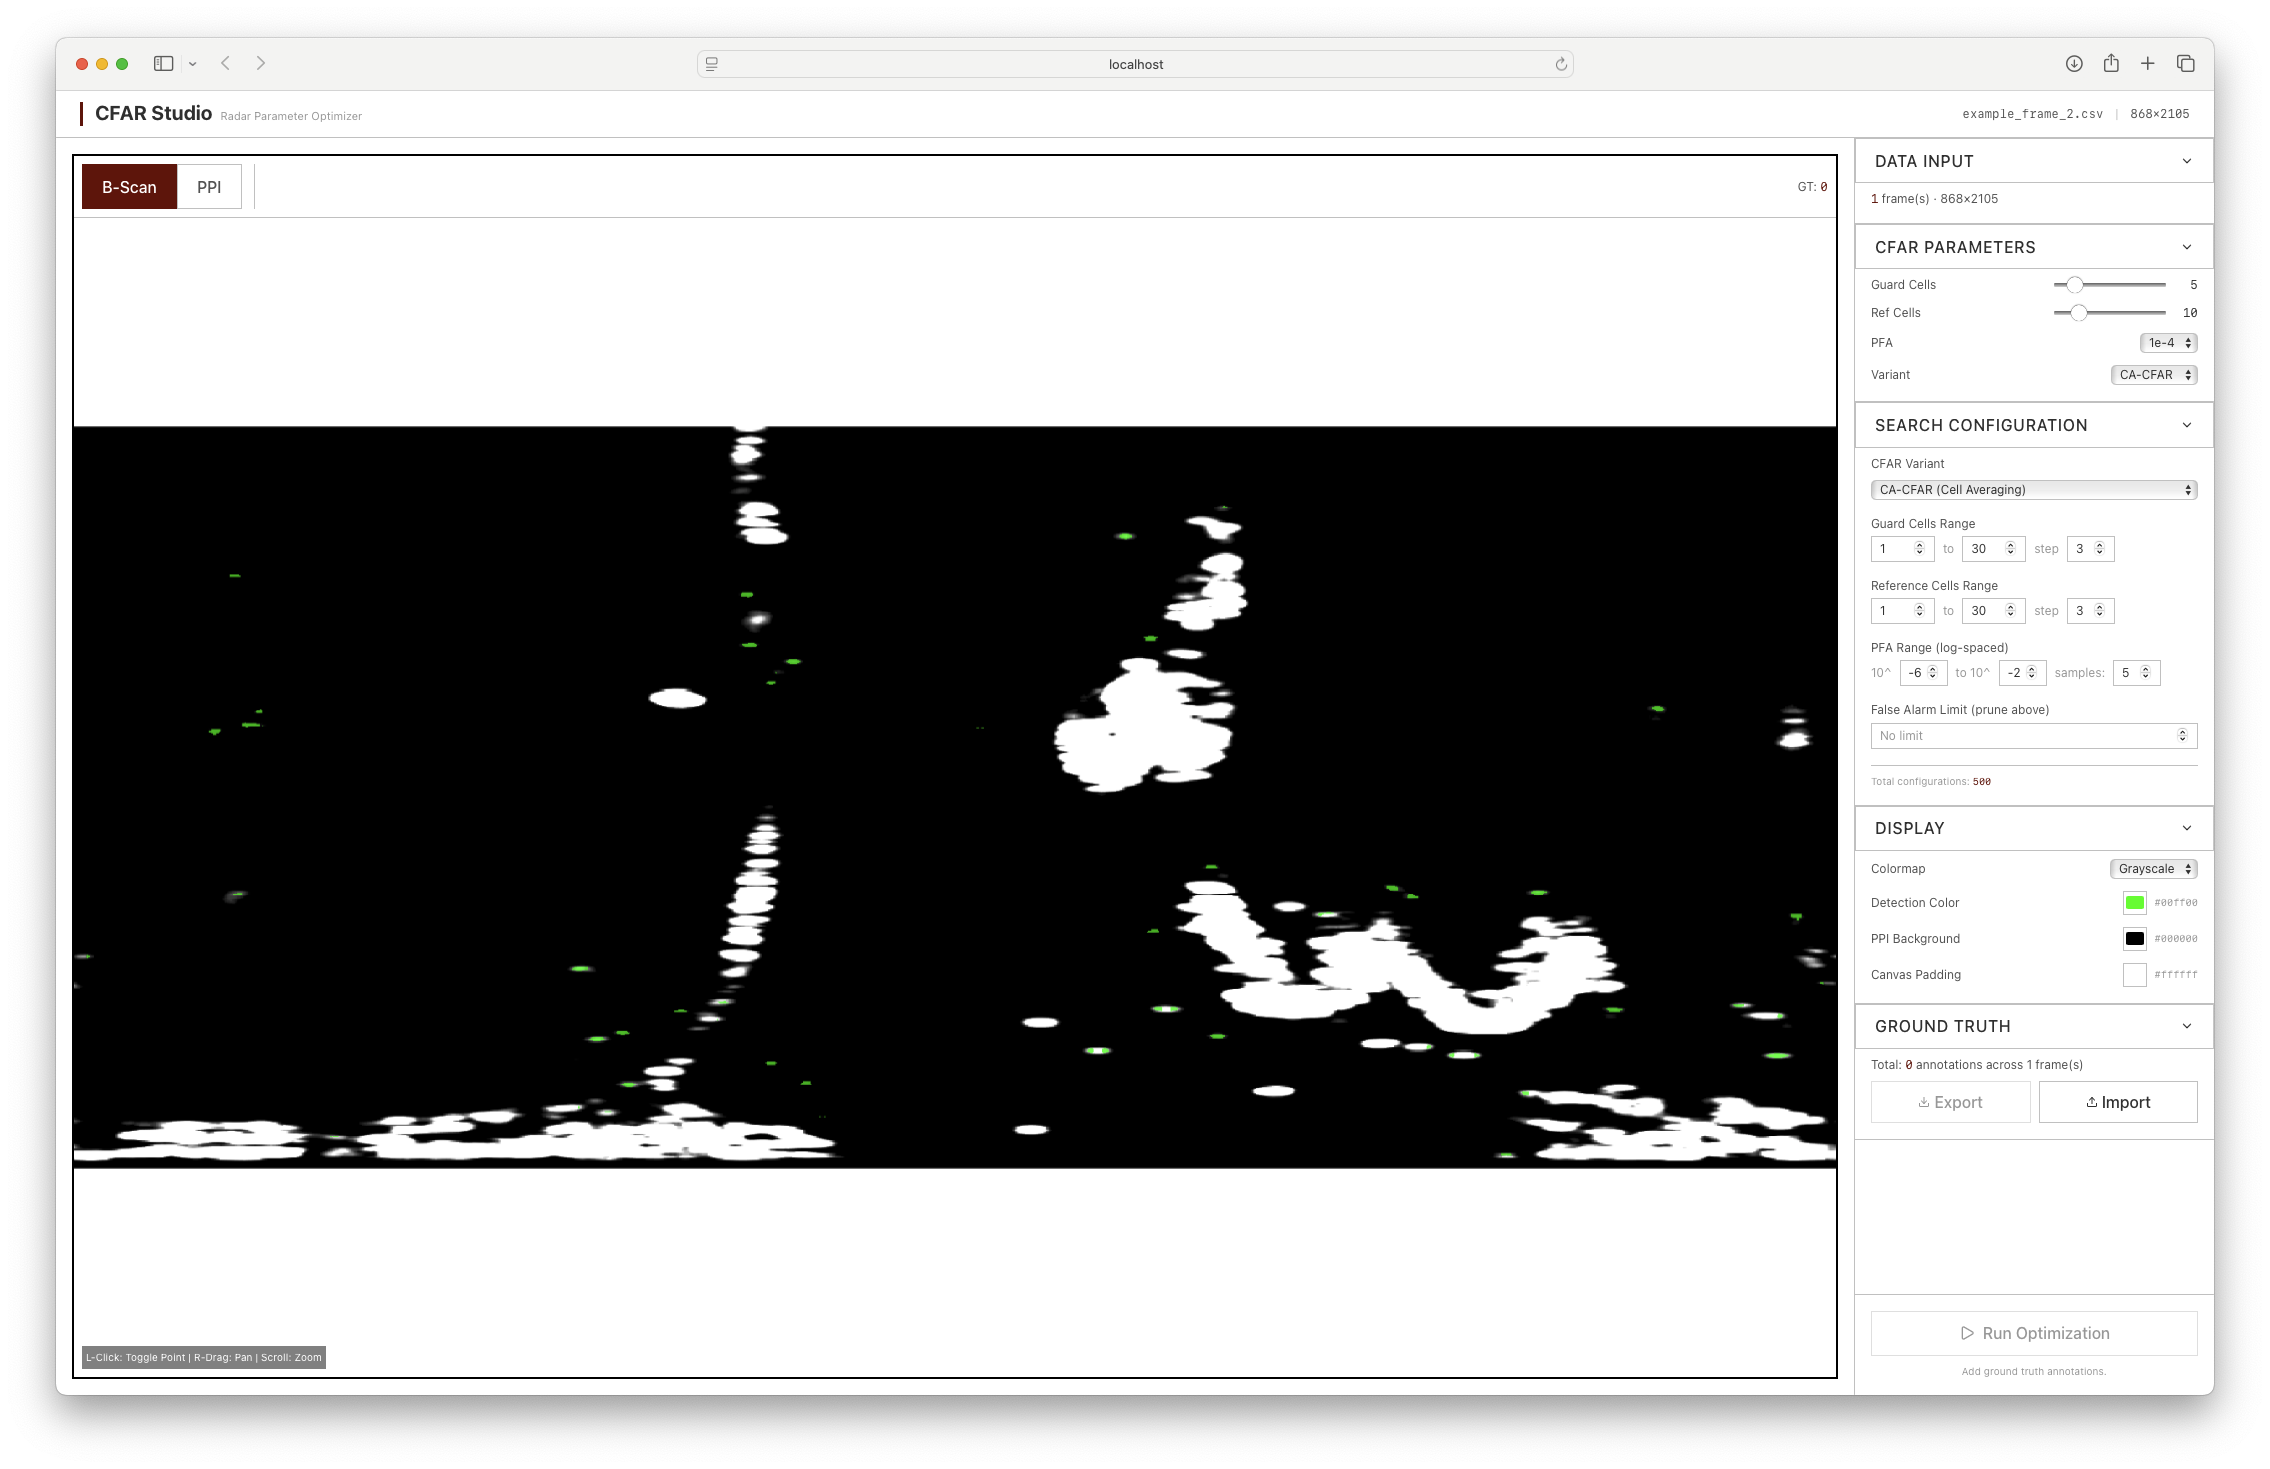
\includegraphics[width=0.95\textwidth, height=2.3cm, keepaspectratio]{Kirk_CFAR_Autotuning/figures/bscan_view_grayscale_with_cfar_detections.png}
      \vspace{-0.3em}
      {\scriptsize B-scan with CFAR detection overlay}
    \end{column}
    \begin{column}{0.52\textwidth}
      \begin{block}{Scoring Function}
        {\scriptsize Coverage ratio and frame score:}
        \vspace{-0.5em}
        \[
          \rho_k = \frac{\textstyle\sum_{p \in B_k} D_t(p)}{|B_k|} \quad S = 0.7\min_k s_k + 0.3\bar{s}
        \]
        \vspace{-0.5em}
      \end{block}
      \vspace{-0.1em}
      \begin{block}{Key Findings}
        {\scriptsize
        \begin{itemize}\setlength{\itemsep}{0pt}\setlength{\topsep}{0pt}
          \item Guard cells $N_g \geq 3$: better extended targets
          \item Optimal reference: $N_r \in [10, 20]$
          \item Top configs: stability $> 0.9$
          \item \textbf{GO-CFAR:} fewest FA near clutter
          \item \textbf{SO-CFAR:} highest detection, more FA
          \item \textbf{CA-CFAR:} best in homogeneous scenes
        \end{itemize}
        }
      \end{block}
    \end{column}
  \end{columns}
\end{frame}

% --- CFAR Pipeline ---
\begin{frame}{CFAR Autotuning -- Processing Pipeline}
  \centering
  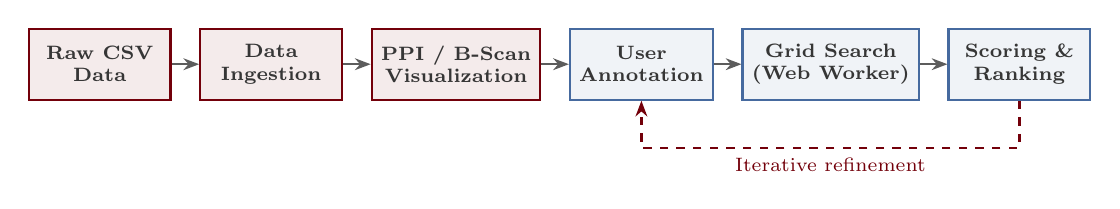
\begin{tikzpicture}[
    pbox/.style={rectangle, draw=Garnet, fill=Garnet!8, line width=0.8pt,
                  minimum height=0.9cm, minimum width=1.8cm,
                  font=\scriptsize\bfseries, align=center, text=Black90},
    sbox/.style={rectangle, draw=Atlantic, fill=Atlantic!8, line width=0.8pt,
                  minimum height=0.9cm, minimum width=1.8cm,
                  font=\scriptsize\bfseries, align=center, text=Black90},
    arr/.style={-{Stealth[length=2mm]}, thick, color=Black70},
    node distance=0.35cm
  ]
    \node[pbox] (csv) {Raw CSV\\Data};
    \node[pbox, right=of csv] (ing) {Data\\Ingestion};
    \node[pbox, right=of ing] (viz) {PPI / B-Scan\\Visualization};
    \node[sbox, right=of viz] (ann) {User\\Annotation};
    \node[sbox, right=of ann] (gs) {Grid Search\\(Web Worker)};
    \node[sbox, right=of gs] (score) {Scoring \&\\Ranking};

    \draw[arr] (csv) -- (ing);
    \draw[arr] (ing) -- (viz);
    \draw[arr] (viz) -- (ann);
    \draw[arr] (ann) -- (gs);
    \draw[arr] (gs) -- (score);
    \draw[arr, dashed, Garnet] (score.south) -- ++(0,-0.6) -| (ann.south)
      node[pos=0.25, below, font=\scriptsize, text=Garnet] {Iterative refinement};
  \end{tikzpicture}

  \vspace{0.3em}
  \begin{columns}[T]
    \begin{column}{0.32\textwidth}
      \begin{block}{CA-CFAR}
        \vspace{-0.3em}
        \[\scriptstyle Z^{CA} = \frac{1}{N}(S_{\text{out}} - S_{\text{in}})\]
        \vspace{-0.5em}
        {\scriptsize Average of all ref.\ cells}
      \end{block}
    \end{column}
    \begin{column}{0.32\textwidth}
      \begin{block}{GO-CFAR}
        \vspace{-0.3em}
        \[\scriptstyle Z^{GO} = \max(\bar{Z}_1, \bar{Z}_2)\]
        \vspace{-0.5em}
        {\scriptsize Greatest-of two halves}
      \end{block}
    \end{column}
    \begin{column}{0.32\textwidth}
      \begin{block}{SO-CFAR}
        \vspace{-0.3em}
        \[\scriptstyle Z^{SO} = \min(\bar{Z}_1, \bar{Z}_2)\]
        \vspace{-0.5em}
        {\scriptsize Smallest-of two halves}
      \end{block}
    \end{column}
  \end{columns}
  \vspace{0.1em}
  {\tiny\textbf{Detection:} $D_t(i,j) = \mathbf{1}[I_t(i,j) > \alpha \cdot Z_{i,j}]$ \enspace $\alpha = N(P_{FA}^{-1/N} - 1)$}
\end{frame}

% =============================================================================
% PAPER 3 -- CANCILLA: ST-DBSCAN
% =============================================================================
\begin{frame}[plain]
  \begin{tikzpicture}[remember picture, overlay]
    \fill[Garnet] (current page.south west) rectangle (current page.north east);
    \node[anchor=center, text=white, font=\Huge\bfseries, text width=14cm, align=center]
      at ([yshift=0.5cm]current page.center) {Paper 3};
    \node[anchor=center, text=Black30, font=\large, text width=14cm, align=center]
      at ([yshift=-1.2cm]current page.center) {Surface-Object Detection and Tracking\\Using Adaptive ST-DBSCAN\\[0.3em]\normalsize S. Cancilla, J.C. Vaught, D. Cahl, Y. Wang};
  \end{tikzpicture}
\end{frame}

% --- Pipeline + Sample ---
\begin{frame}{Adaptive ST-DBSCAN -- Approach}
  \begin{columns}[T]
    \begin{column}{0.50\textwidth}
      \begin{block}{Pipeline}
        \centering
        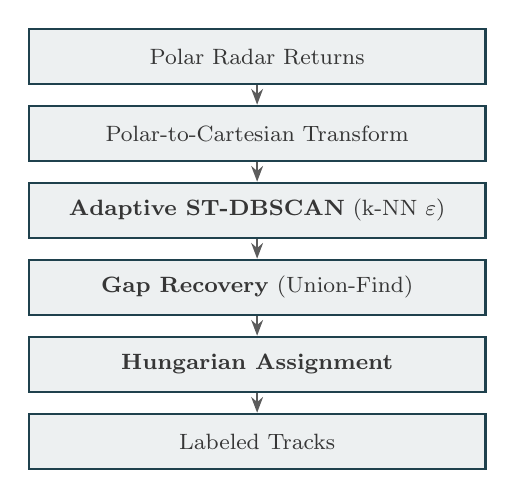
\begin{tikzpicture}[
          pbox/.style={rectangle, draw=Congaree, fill=Congaree!8, line width=0.8pt,
                        minimum height=0.7cm, minimum width=5.8cm,
                        font=\footnotesize, align=center, text=Black90},
          arr/.style={-{Stealth[length=2mm]}, thick, color=Black70},
          node distance=0.25cm
        ]
          \node[pbox] (p1) {Polar Radar Returns};
          \node[pbox, below=of p1] (p2) {Polar-to-Cartesian Transform};
          \node[pbox, below=of p2] (p3) {\textbf{Adaptive ST-DBSCAN} (k-NN $\varepsilon$)};
          \node[pbox, below=of p3] (p4) {\textbf{Gap Recovery} (Union-Find)};
          \node[pbox, below=of p4] (p5) {\textbf{Hungarian Assignment}};
          \node[pbox, below=of p5] (p6) {Labeled Tracks};
          \draw[arr] (p1)--(p2); \draw[arr] (p2)--(p3);
          \draw[arr] (p3)--(p4); \draw[arr] (p4)--(p5);
          \draw[arr] (p5)--(p6);
        \end{tikzpicture}
      \end{block}
    \end{column}
    \begin{column}{0.47\textwidth}
      \begin{block}{Key Innovations}
        {\scriptsize
        \begin{itemize}\setlength{\itemsep}{0pt}\setlength{\topsep}{0pt}
          \item \textbf{Adaptive $\varepsilon$:} k-NN distance statistics
            \vspace{-0.4em}
            \[\scriptstyle \varepsilon_s = \max\!\Big(\text{P}_{90}\{d_k\},\; \varepsilon_{\min}\Big) \]
            \vspace{-1em}
          \item \textbf{Gap recovery:} Union-Find merging
            \vspace{-0.4em}
            \[\scriptstyle d_{\max} = v_{\max} \cdot \Delta t \cdot T_s \]
            \vspace{-1em}
          \item \textbf{Hungarian assignment:} optimal track association
        \end{itemize}
        }
      \end{block}
      \vspace{-0.15em}
      \begin{block}{Implementation}
        \vspace{-0.15em}
        {\scriptsize Rust + Rayon (data-parallel k-NN)\\
        Spatial hashing: $h = 2\varepsilon_{\max}$\\
        Target: NVIDIA Jetson AGX Orin}
        \vspace{-0.15em}
      \end{block}
    \end{column}
  \end{columns}
\end{frame}

% --- Clustering Comparison ---
\begin{frame}{Adaptive ST-DBSCAN -- Clustering Comparison}
  \begin{columns}[c]
    \begin{column}{0.32\textwidth}
      \centering
      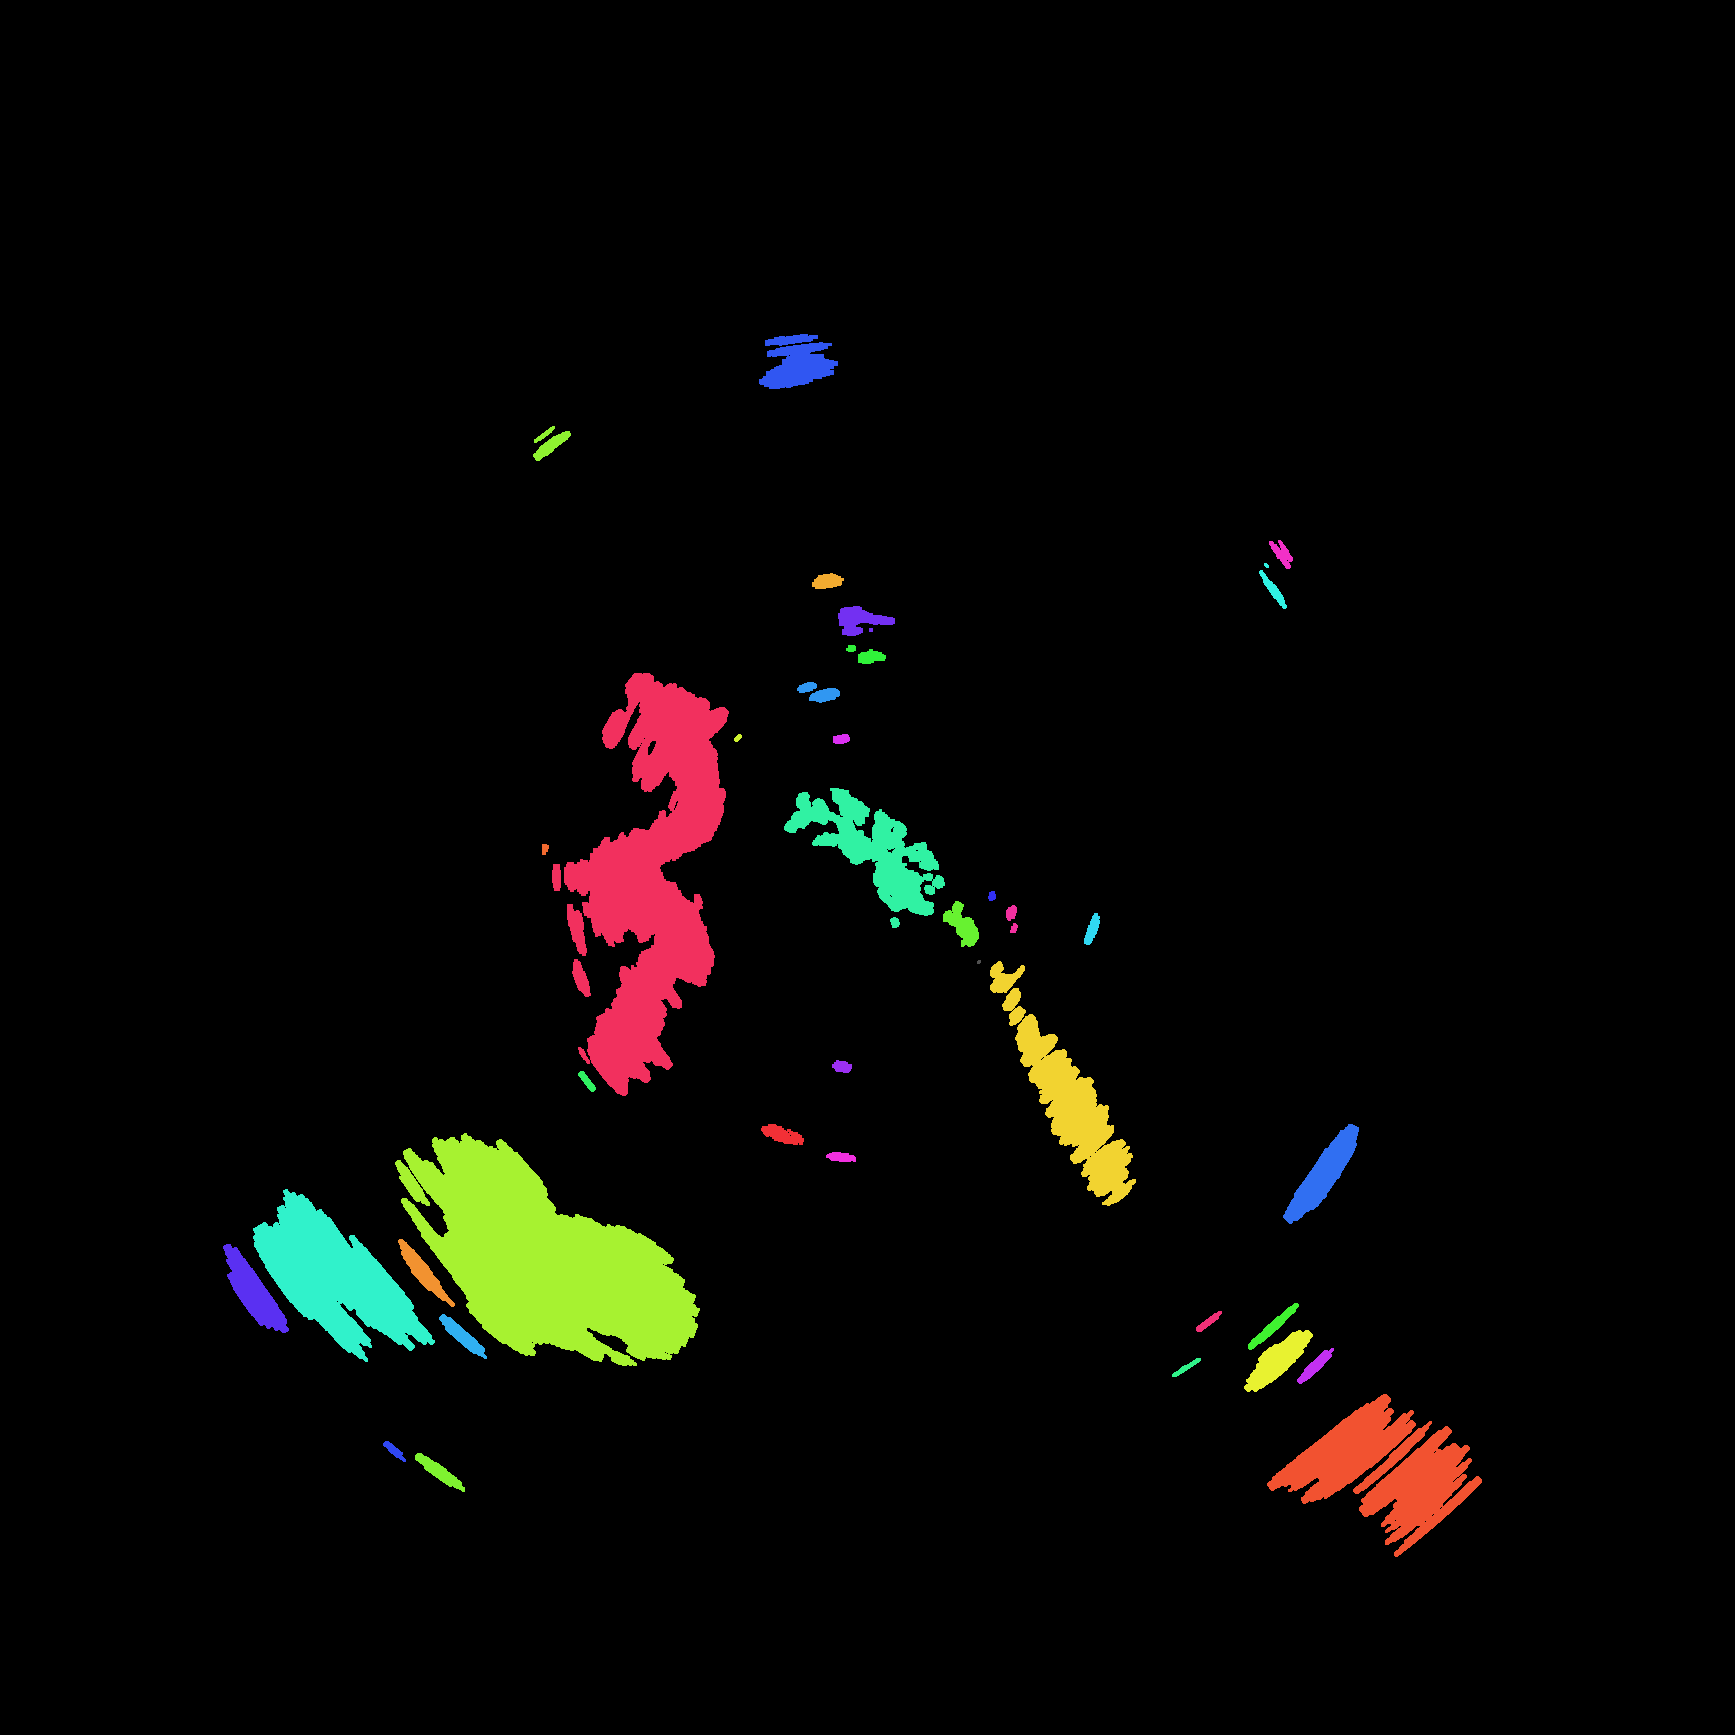
\includegraphics[width=\textwidth]{Cancilla_ST-DBSCAN/figures/dbscan_frame.png}
      {\scriptsize\textbf{Vanilla DBSCAN}\\1693 clusters (over-segmented)}
    \end{column}
    \begin{column}{0.32\textwidth}
      \centering
      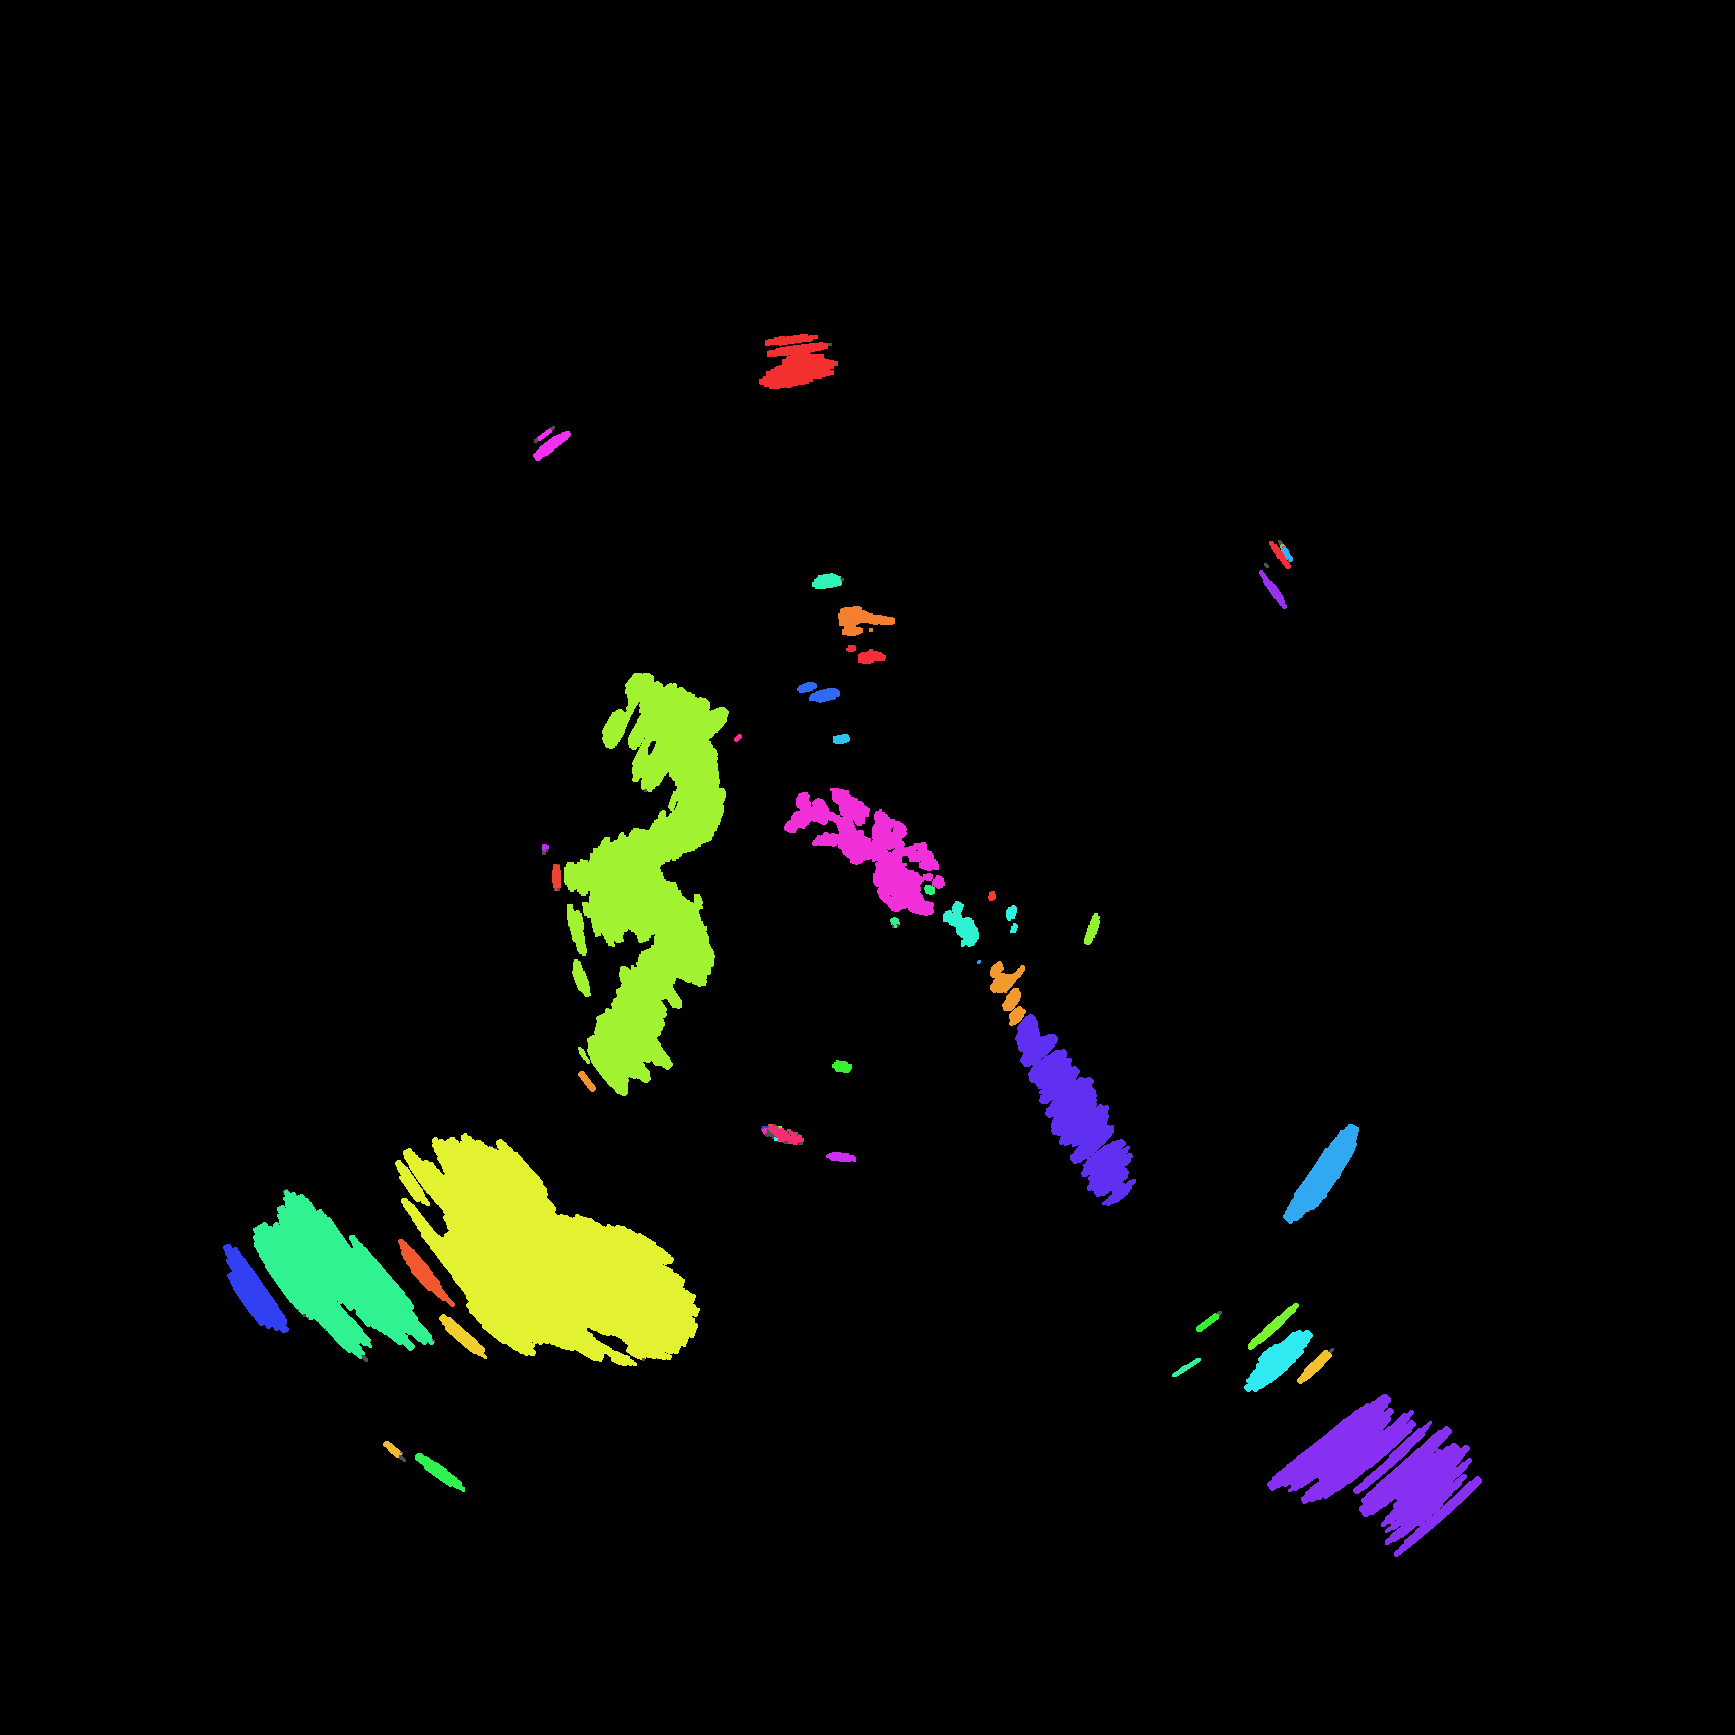
\includegraphics[width=\textwidth]{Cancilla_ST-DBSCAN/figures/stdbscan_frame.png}
      {\scriptsize\textbf{Adaptive ST-DBSCAN}\\1177 clusters (reduced noise)}
    \end{column}
    \begin{column}{0.32\textwidth}
      \centering
      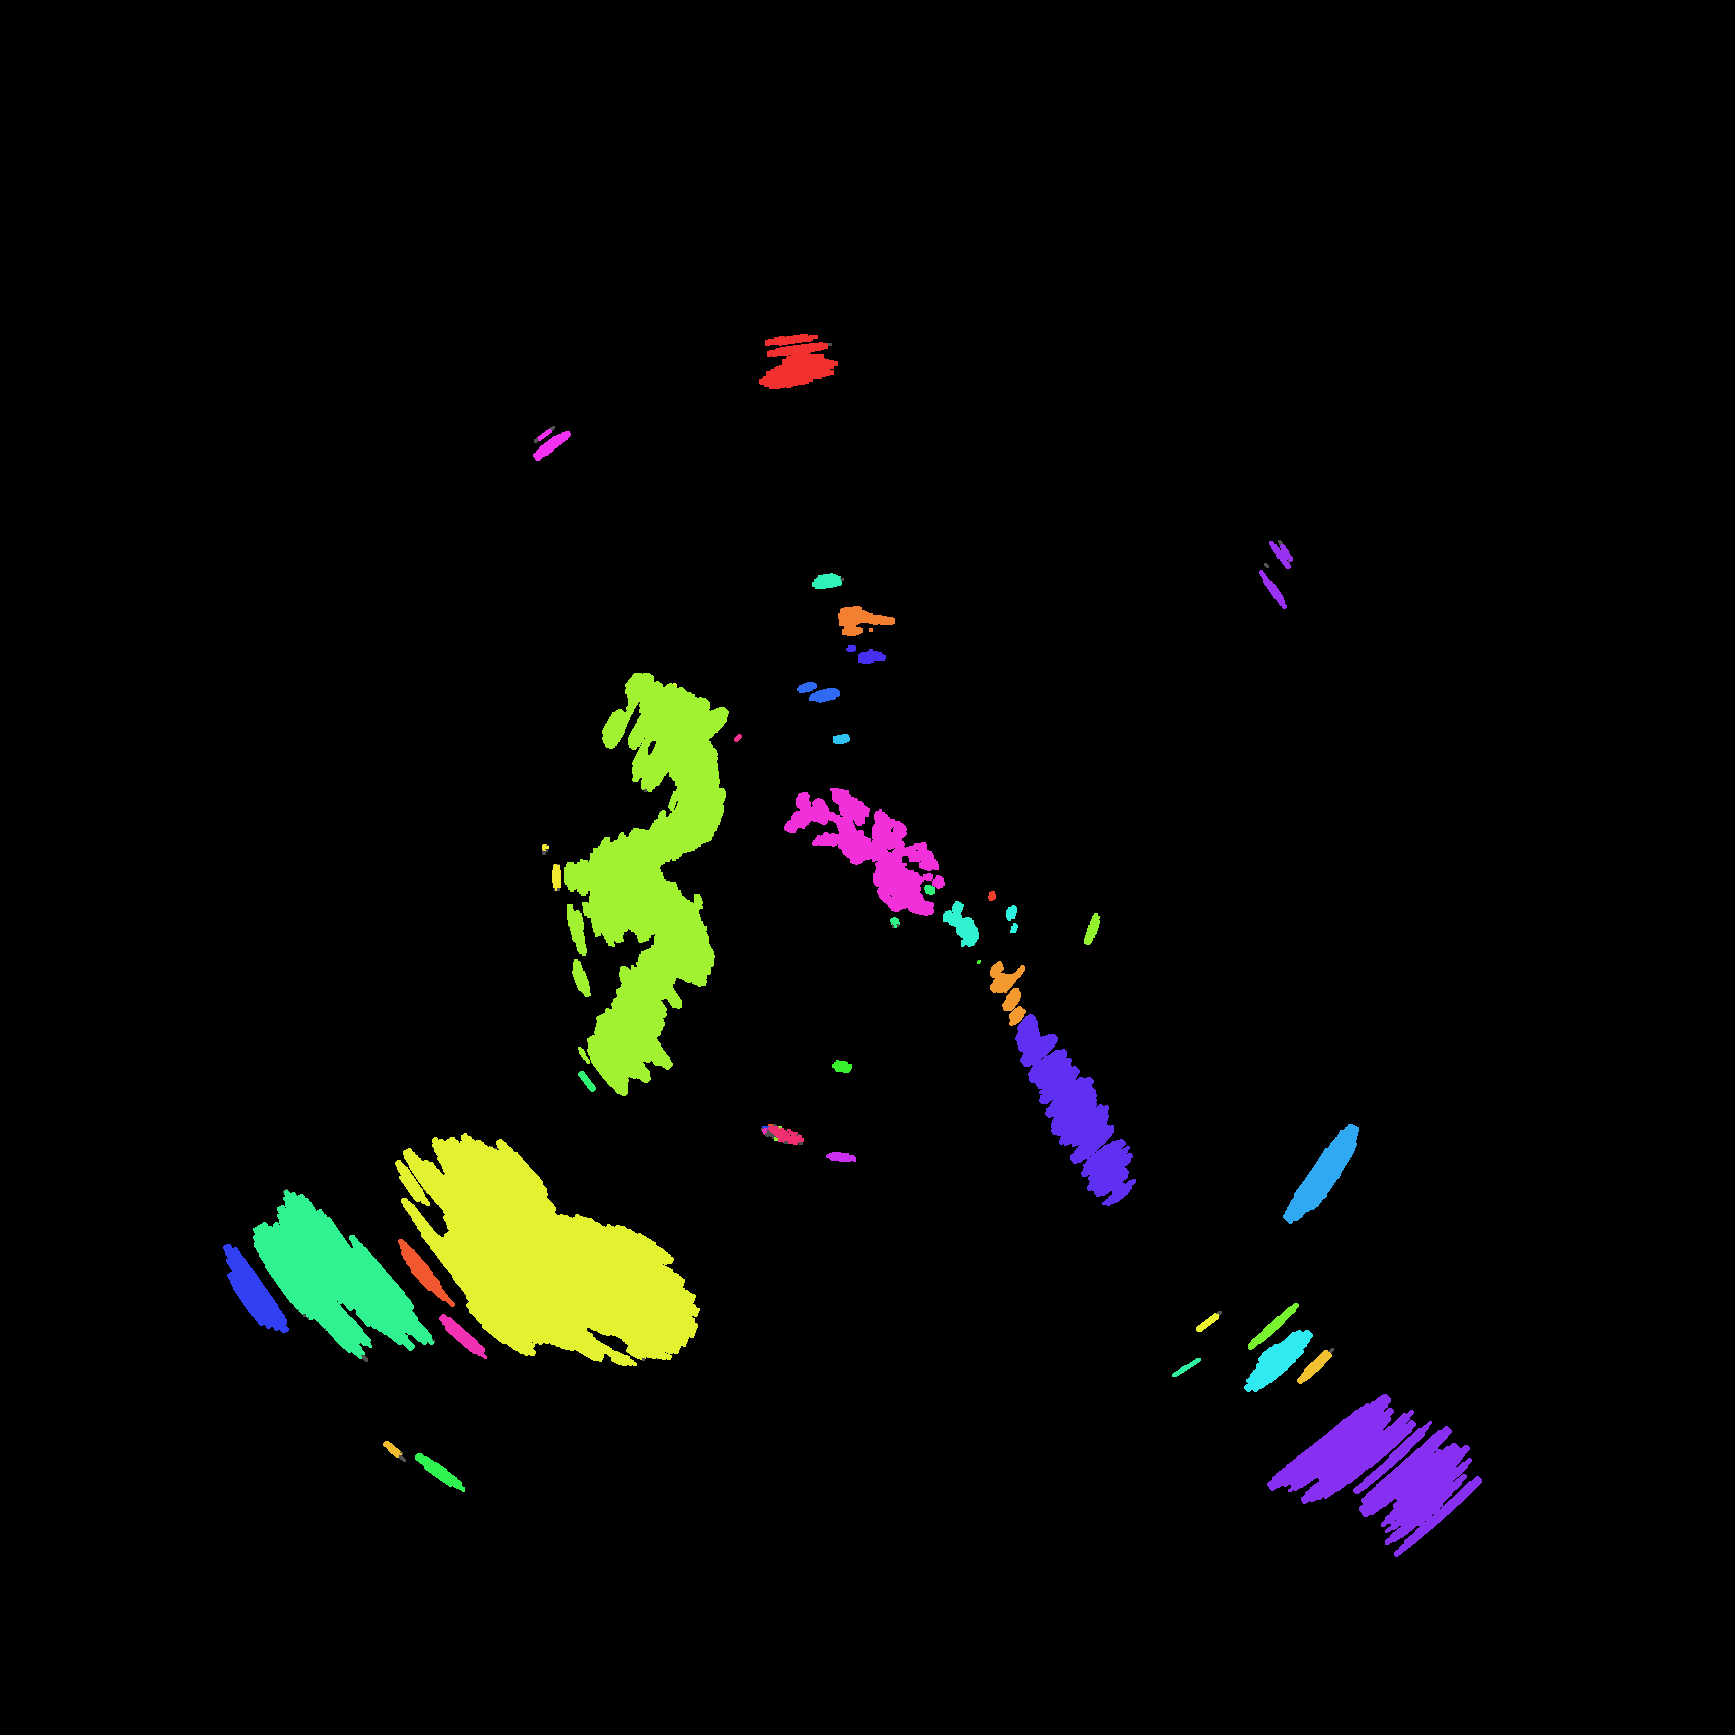
\includegraphics[width=\textwidth]{Cancilla_ST-DBSCAN/figures/gap_frame.png}
      {\scriptsize\textbf{+ Gap Recovery}\\Consolidated track fragments}
    \end{column}
  \end{columns}
  \vspace{0.5em}
  \centering
  {\small Synthetic X-band radar data -- compound K-distribution clutter with Bernoulli flicker model (15--40\% dropout)}
\end{frame}

% --- Tracking Results ---
\begin{frame}{Adaptive ST-DBSCAN -- Tracking Results}
  \begin{columns}[T]
    \begin{column}{0.42\textwidth}
      \centering
      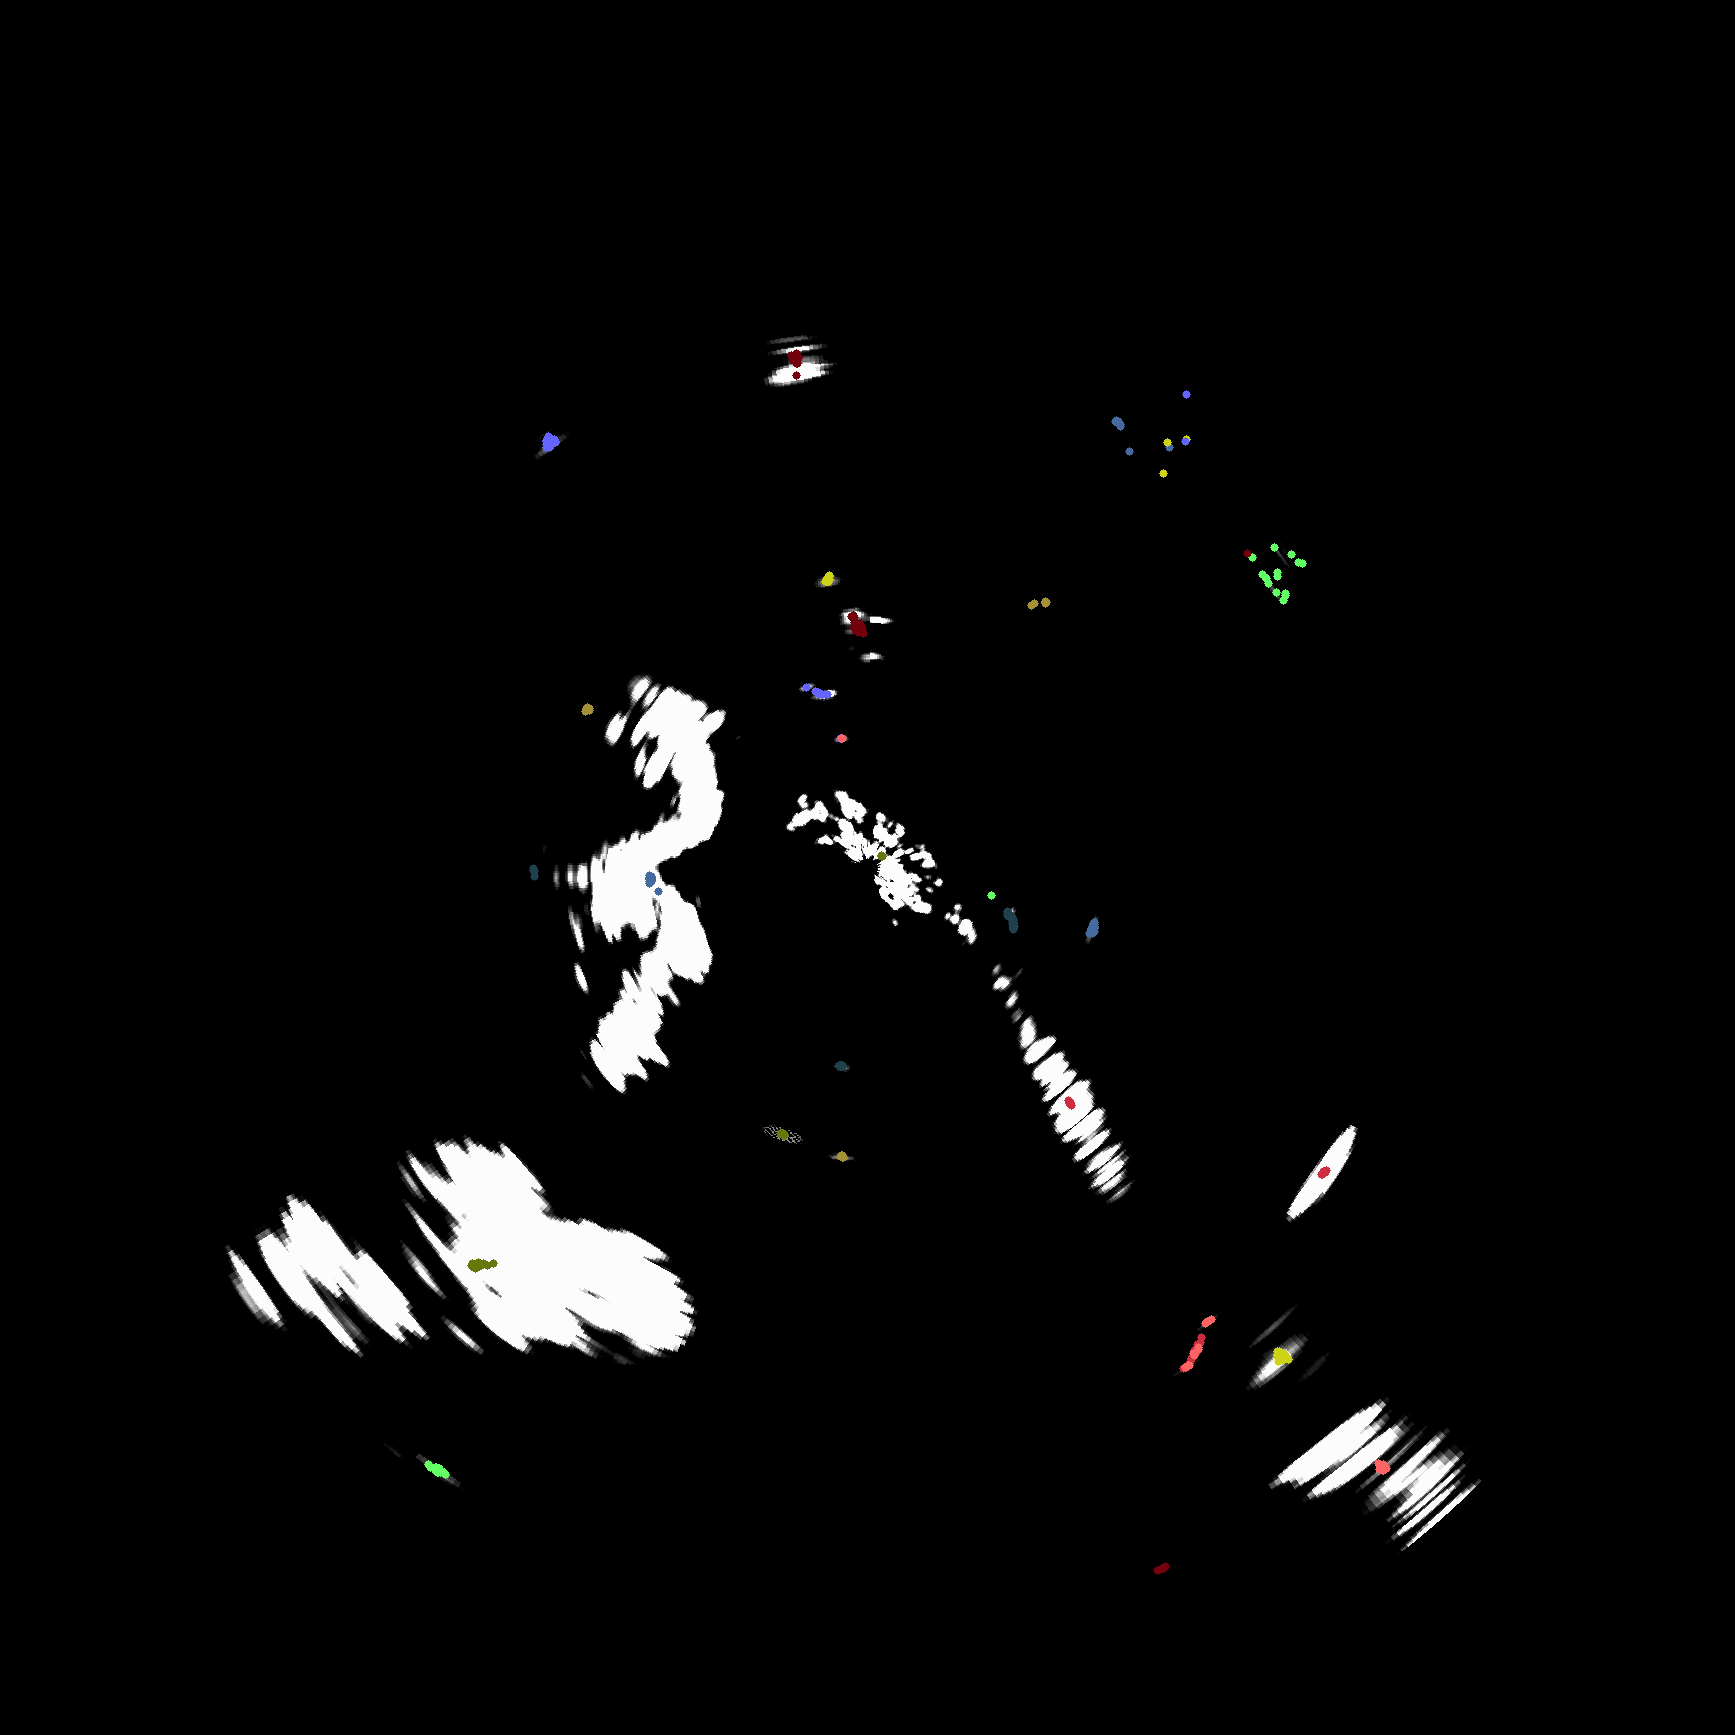
\includegraphics[width=0.95\textwidth]{Cancilla_ST-DBSCAN/figures/gap_track_frame.png}
      \vspace{-0.3em}
      {\scriptsize Final tracking: 3 objects with stable IDs}
    \end{column}
    \begin{column}{0.55\textwidth}
      \begin{block}{MOT Metrics Comparison}
        \centering
        \tiny
        \renewcommand{\arraystretch}{1.0}
        \begin{tabular}{@{}l c c c c@{}}
          \toprule
          \textbf{Method} & \textbf{MOTA} & \textbf{MOTP} & \textbf{Recall} & \textbf{IDSW} \\
          \midrule
          Vanilla DBSCAN & $-6.97$ & 1.80 & 0.987 & 18 \\
          Std.\ ST-DBSCAN & $-0.10$ & --- & 0.000 & 0 \\
          \rowcolor{Garnet!10}
          Adaptive ST-DBSCAN & $\mathbf{-4.44}$ & $\mathbf{1.19}$ & $\mathbf{0.974}$ & 18 \\
          \rowcolor{Congaree!10}
          + Gap Recovery & $-3.82$ & 1.18 & 0.812 & $\mathbf{0}$ \\
          \bottomrule
        \end{tabular}
      \end{block}
      \vspace{-0.1em}
      \begin{block}{Edge Performance (Jetson AGX Orin)}
        \centering
        \tiny
        \renewcommand{\arraystretch}{0.95}
        \begin{tabular}{@{}l r@{}}
          \toprule
          \textbf{Stage} & \textbf{Time (ms)} \\
          \midrule
          Adaptive $\varepsilon$ (k-NN) & 196 \\
          ST-DBSCAN clustering & 169 \\
          Gap recovery + extraction & 53 \\
          Hungarian + I/O & 50 \\
          \midrule
          \textbf{Total} & \textbf{511 $\pm$ 93} \\
          \bottomrule
        \end{tabular}

        {\scriptsize $\sim$2 sweeps/s $>$ real-time for 48\,RPM radar}
      \end{block}
    \end{column}
  \end{columns}
\end{frame}

% =============================================================================
% PAPER 4 -- WANG: ACTIVE ACQUISITION
% =============================================================================
\begin{frame}[plain]
  \begin{tikzpicture}[remember picture, overlay]
    \fill[Garnet] (current page.south west) rectangle (current page.north east);
    \node[anchor=center, text=white, font=\Huge\bfseries, text width=14cm, align=center]
      at ([yshift=0.5cm]current page.center) {Paper 4};
    \node[anchor=center, text=Black30, font=\large, text width=14cm, align=center]
      at ([yshift=-1.2cm]current page.center) {Dual-Camera Active Acquisition\\for Small-Object Dataset Construction\\[0.3em]\normalsize J. Wang, J.C. Vaught, D. Cahl, Y. Wang};
  \end{tikzpicture}
\end{frame}

% --- Motivation + Hardware ---
\begin{frame}{Dual-Camera Acquisition -- Concept}
  \begin{columns}[T]
    \begin{column}{0.55\textwidth}
      \begin{block}{Digital Zoom vs.\ Super-Resolution vs.\ Optical Zoom}
        \centering
        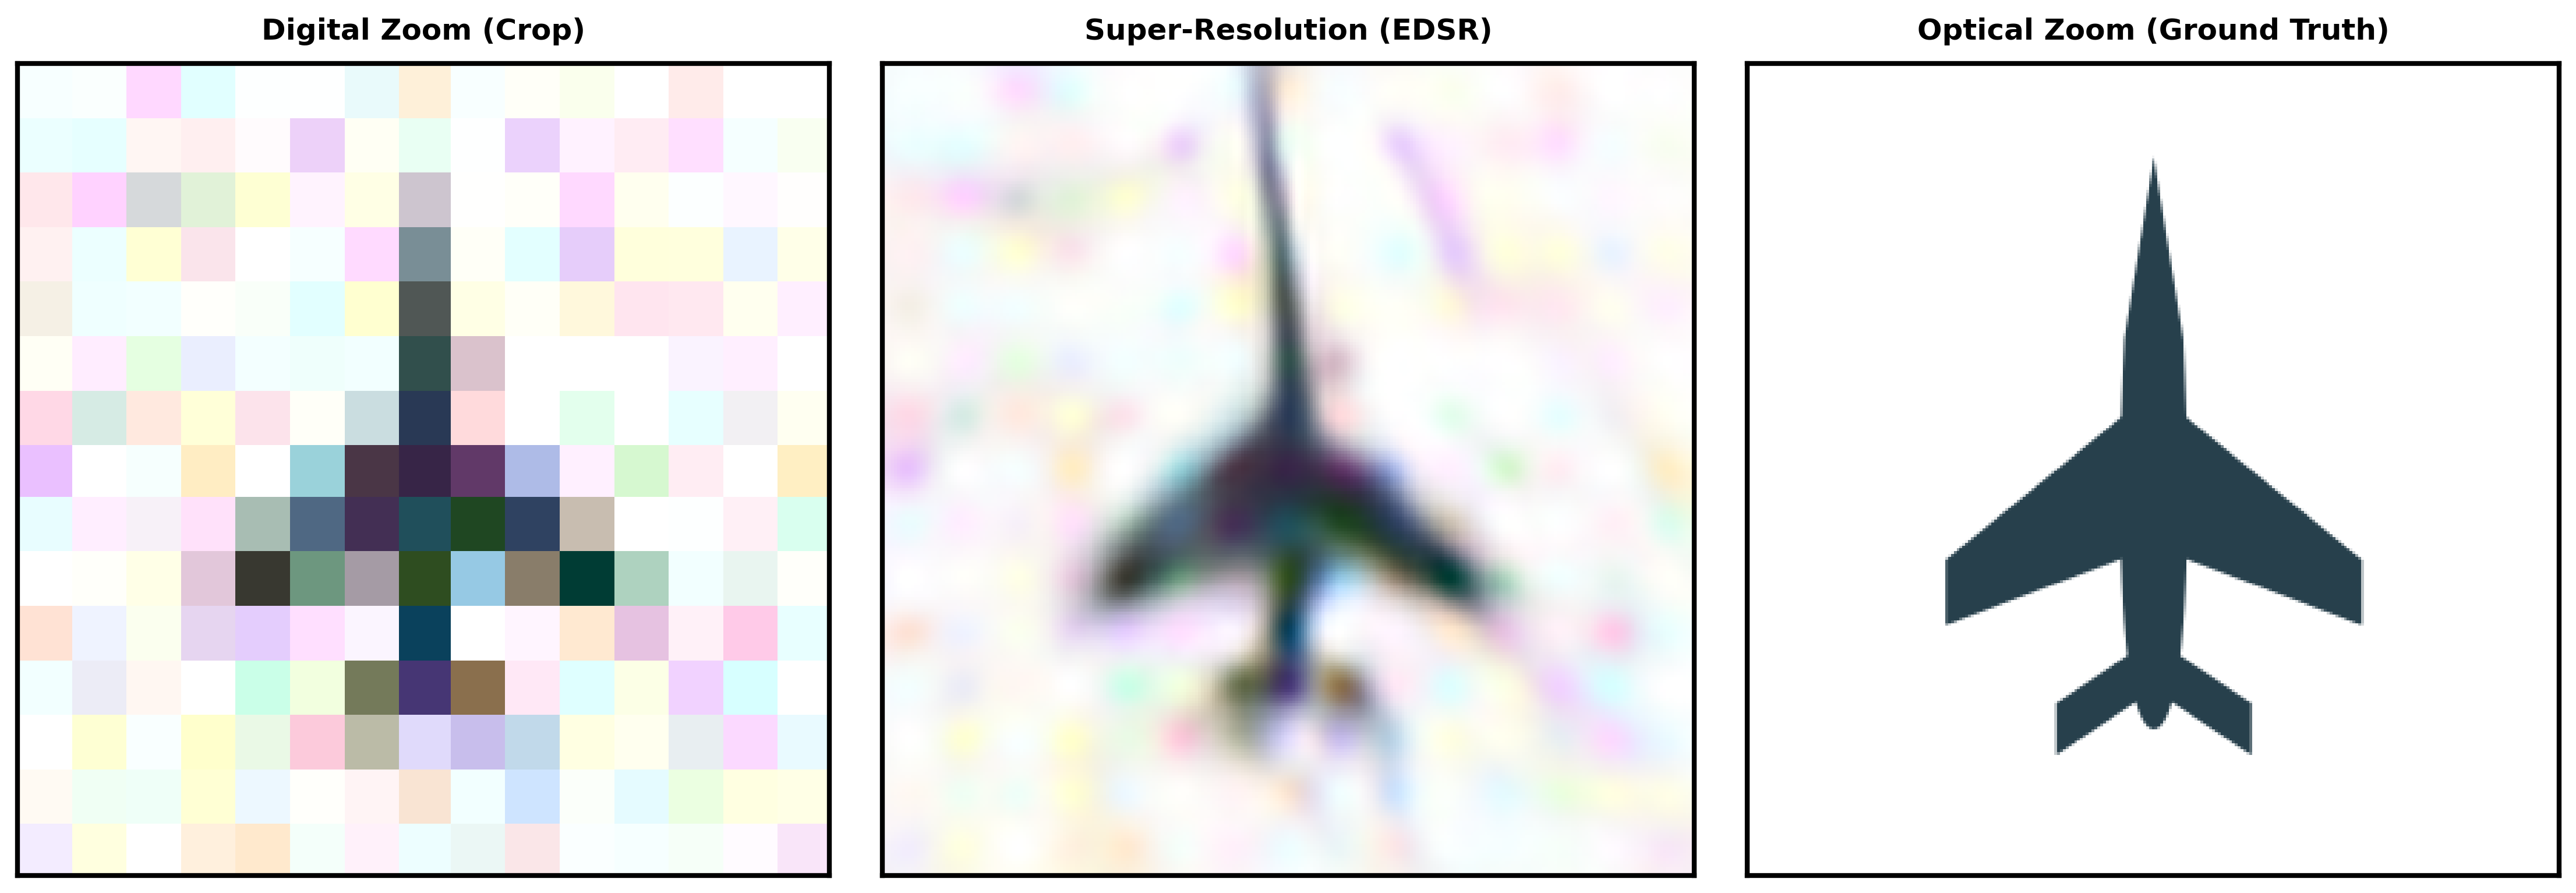
\includegraphics[width=0.90\textwidth, height=2.0cm, keepaspectratio]{Wang_Active_Acquisition/figures/fig_sr_comparison.png}
        \vspace{-0.3em}
        {\tiny Left: pixelated crop $|$ Center: SR hallucination $|$ Right: optical zoom}
      \end{block}
      \vspace{-0.1em}
      \begin{block}{Key Idea}
        {\scriptsize Replace human labelers with a \textbf{dual-camera system}:
        \begin{itemize}\setlength{\itemsep}{0pt}\setlength{\topsep}{0pt}
          \item \textbf{Wide-angle} (fixed): persistent detection coverage
          \item \textbf{PTZ} (steerable): optical zoom verification
          \item Hard small-object detection $\to$ trivial classification
        \end{itemize}
        }
      \end{block}
    \end{column}
    \begin{column}{0.42\textwidth}
      \centering
      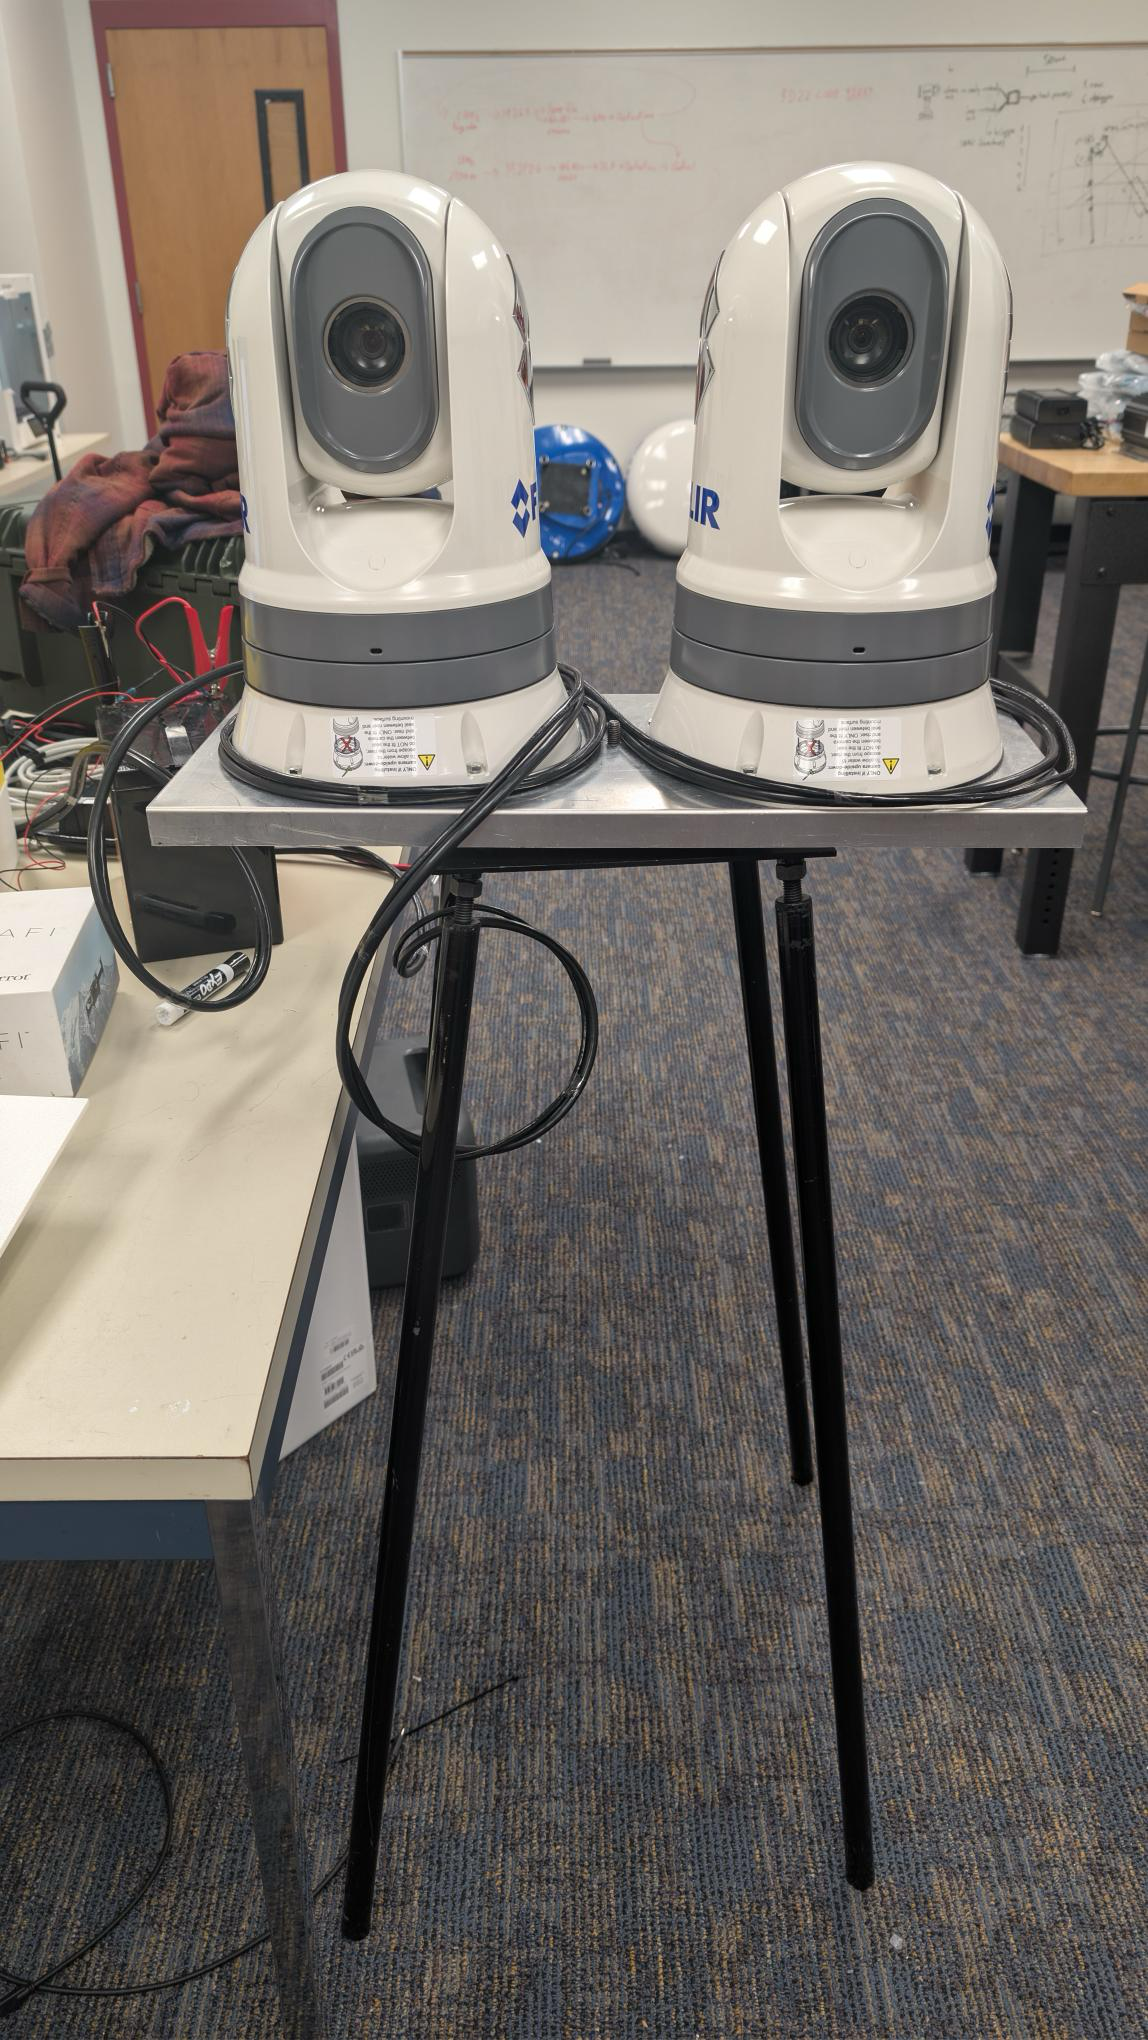
\includegraphics[width=0.45\textwidth, height=2.4cm, keepaspectratio]{Wang_Active_Acquisition/report_images/image_01.png}
      \vspace{-0.3em}
      {\scriptsize 2$\times$ FLIR M300C on 0.9\,m stand}

      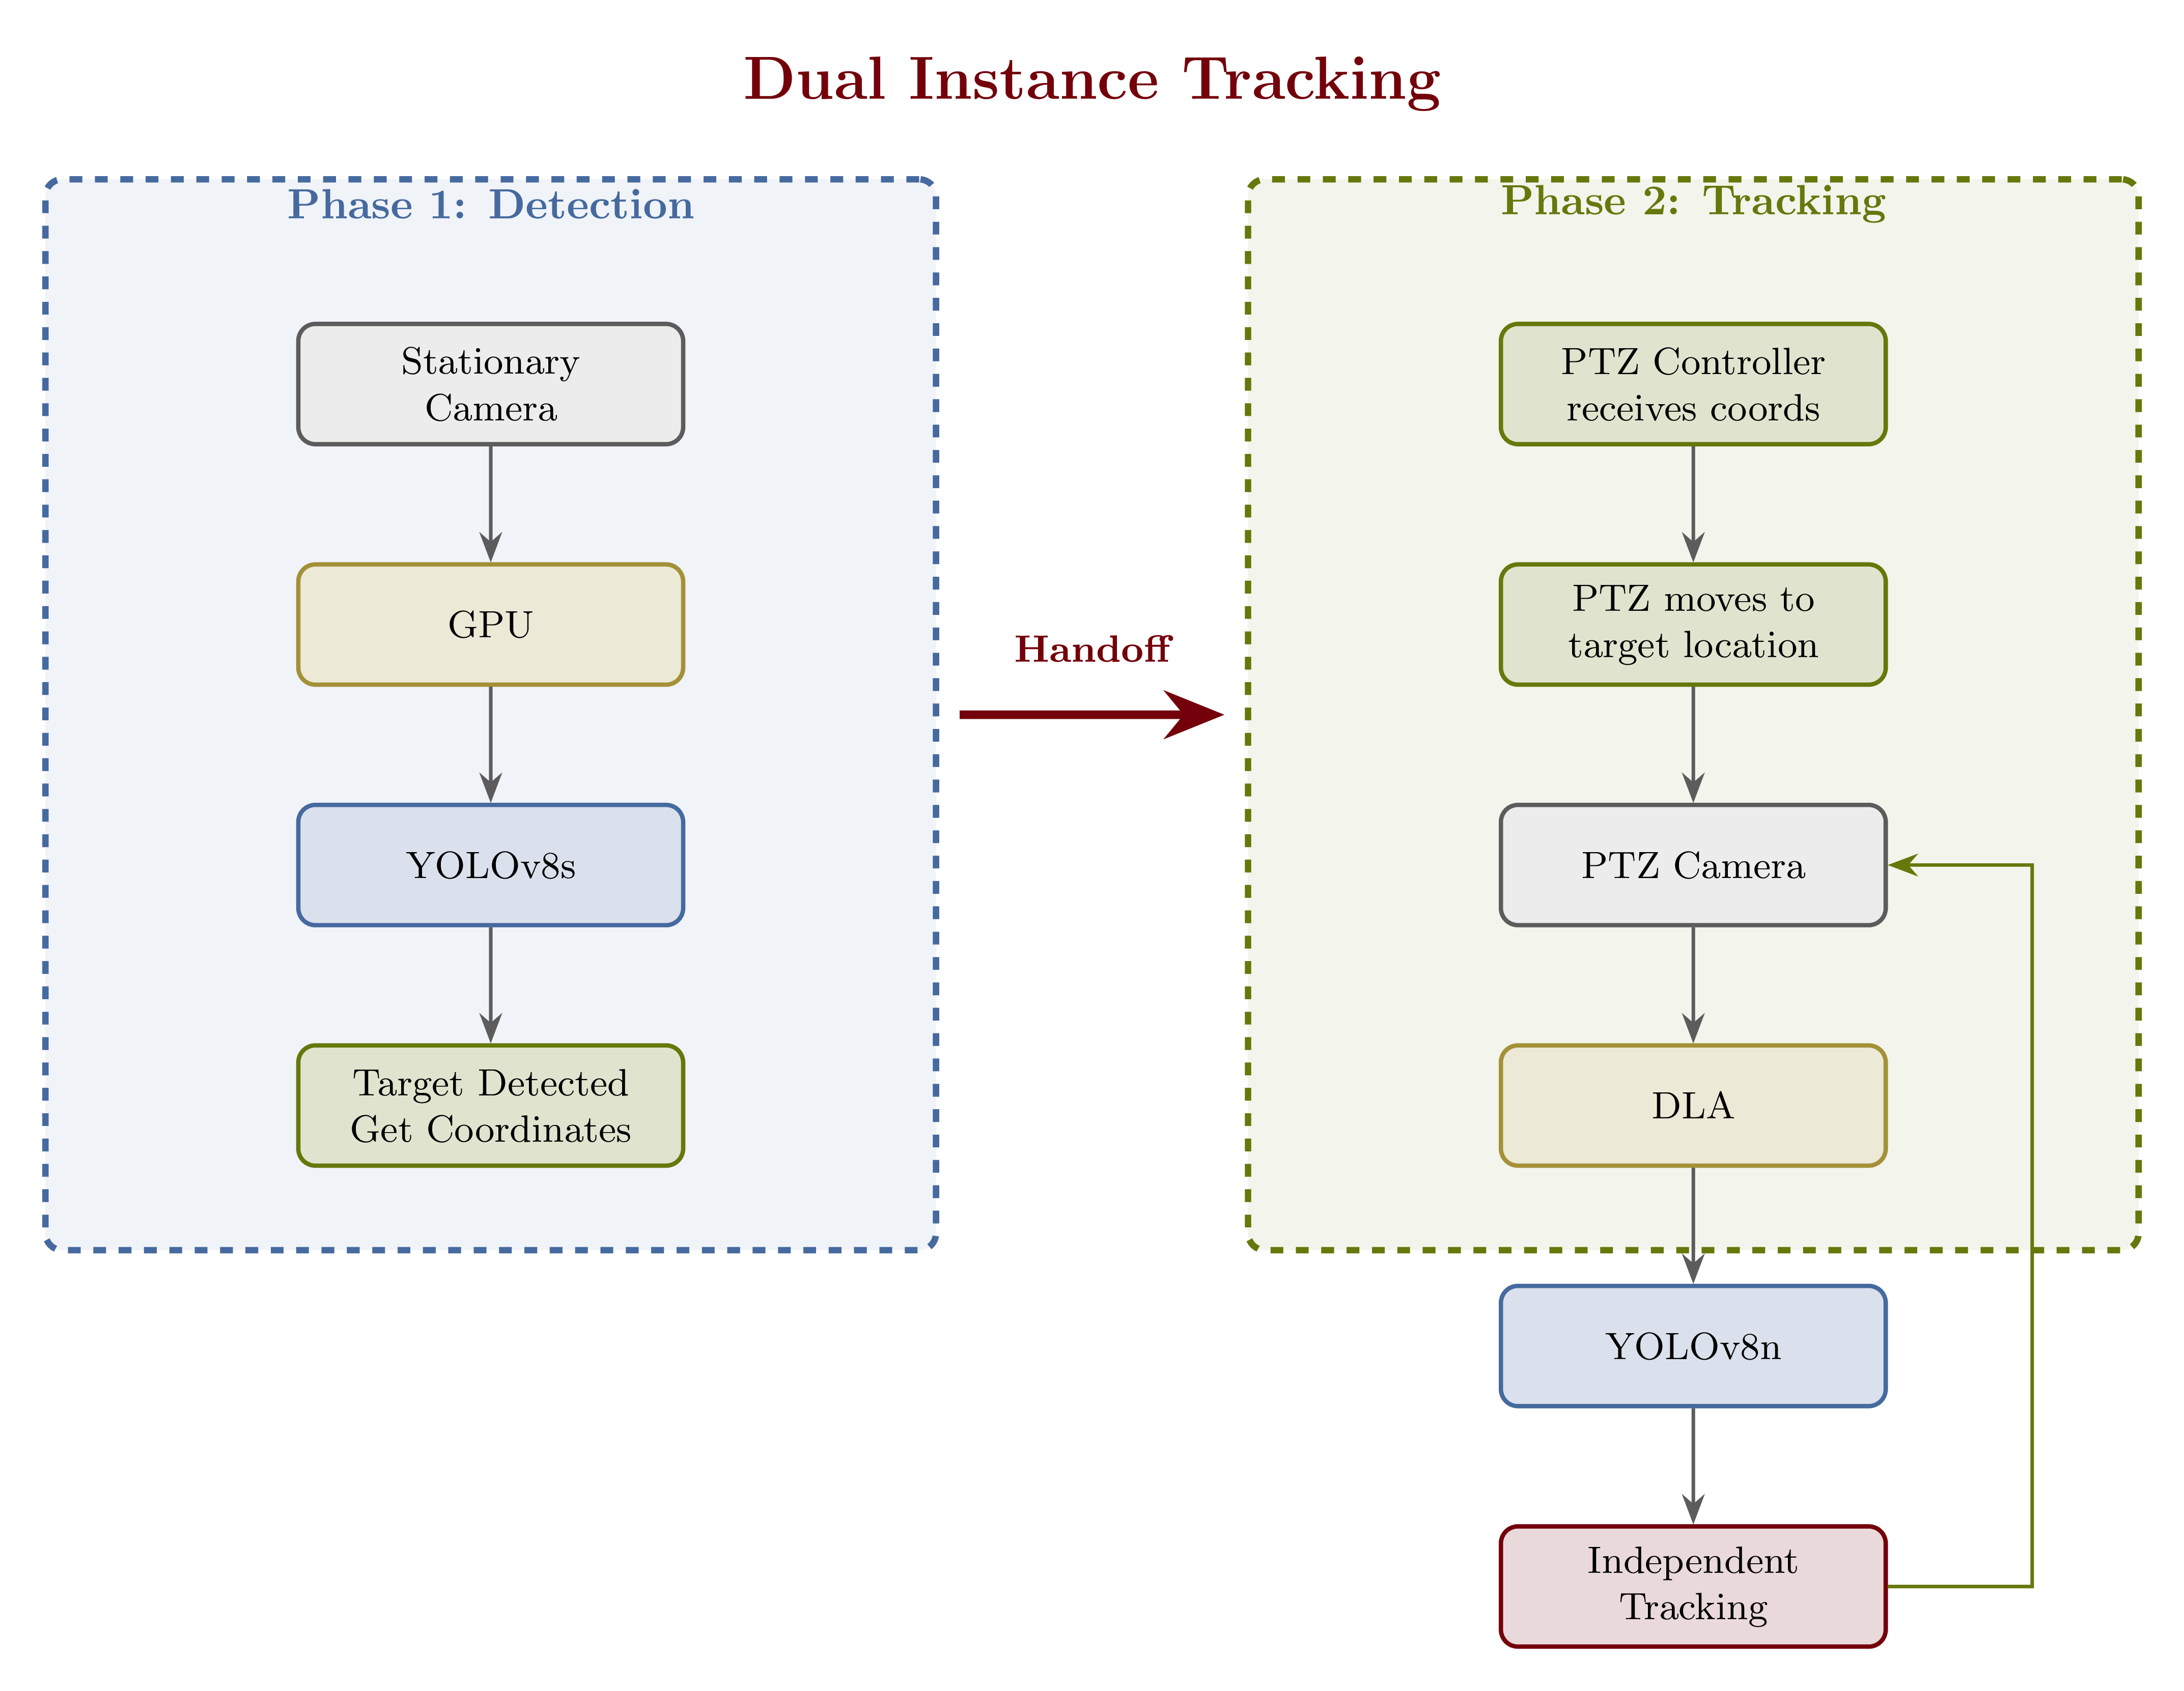
\includegraphics[width=0.85\textwidth, height=2.0cm, keepaspectratio]{Wang_Active_Acquisition/report_images/image_02.png}
      \vspace{-0.3em}
      {\scriptsize Dual-instance tracking pipeline}
    \end{column}
  \end{columns}
\end{frame}

% --- Live Tracking ---
\begin{frame}{Dual-Camera Acquisition -- Drone Tracking Demo}
  \begin{columns}[T]
    \begin{column}{0.50\textwidth}
      \centering
      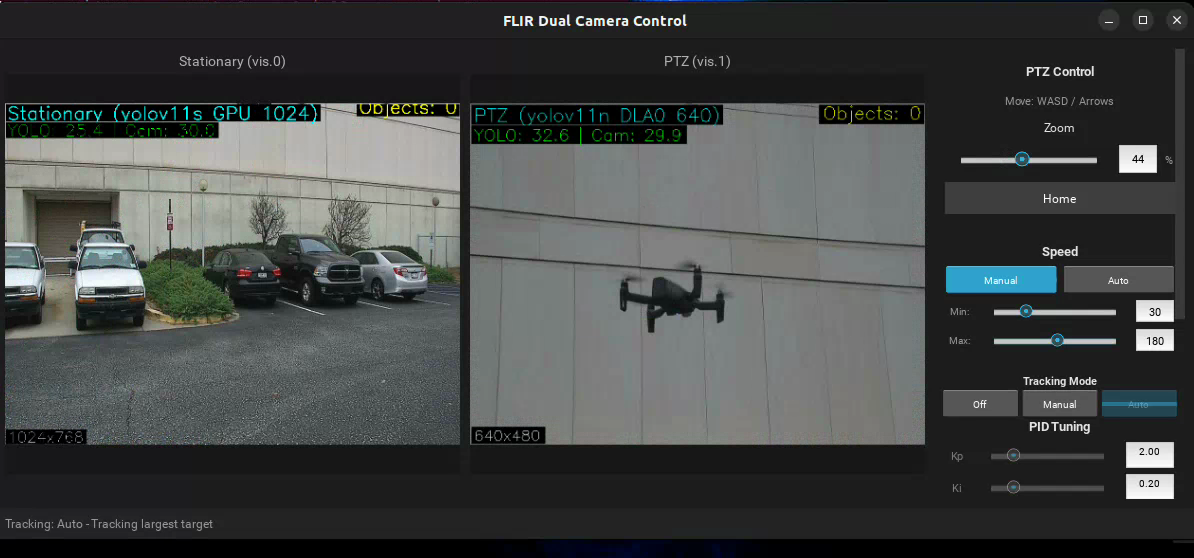
\includegraphics[width=0.95\textwidth, height=2.8cm, keepaspectratio]{Wang_Active_Acquisition/figures/fig_gui_dual_feed.png}
      \vspace{-0.3em}
      {\scriptsize Wide-angle: $\sim$20$\times$15\,px target (GPU, YOLOv11s)}

      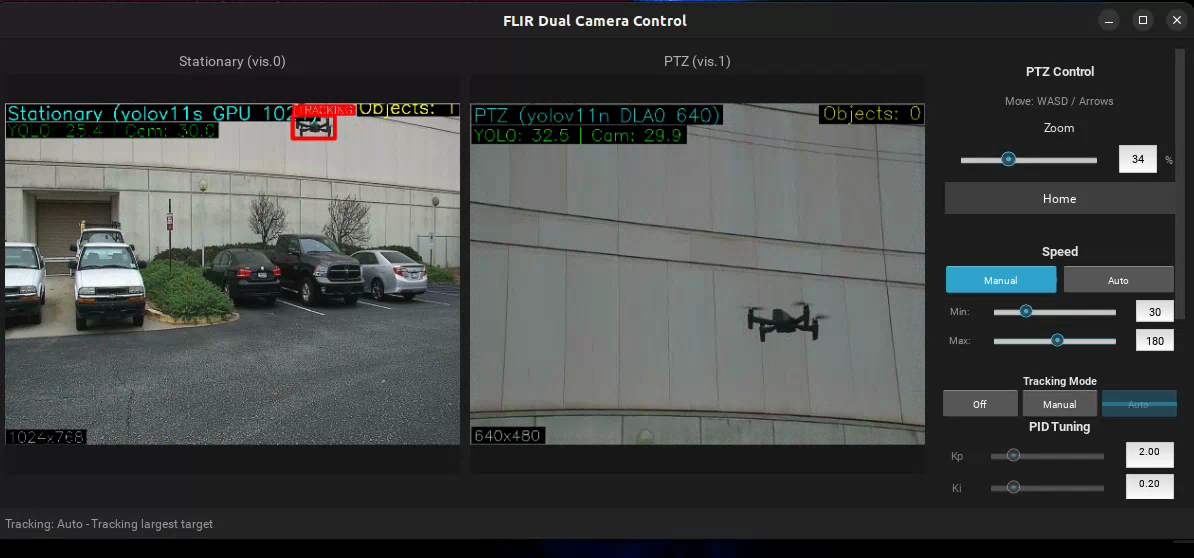
\includegraphics[width=0.95\textwidth, height=2.8cm, keepaspectratio]{Wang_Active_Acquisition/figures/fig_drone_tracking.png}
      \vspace{-0.3em}
      {\scriptsize PTZ zoom: $\sim$120$\times$90\,px (DLA, YOLOv11n) -- 6$\times$ resolution}
    \end{column}
    \begin{column}{0.47\textwidth}
      \begin{block}{Detector Throughput}
        \centering
        \tiny
        \renewcommand{\arraystretch}{0.95}
        \begin{tabular}{@{}l l l@{}}
          \toprule
          & \textbf{Wide (GPU)} & \textbf{PTZ (DLA)} \\
          \midrule
          Model       & YOLOv11s & YOLOv11n \\
          Inference   & 27.9\,ms & 46.5\,ms \\
          Throughput  & 35.9\,FPS & 21.5\,FPS \\
          Detection   & 100\% & 99\% \\
          \bottomrule
        \end{tabular}

        {\scriptsize Aggregate: \textbf{57.4 FPS} (true parallel)}
      \end{block}
      \vspace{-0.1em}
      \begin{block}{Tracking Controller}
        {\scriptsize
        \begin{itemize}\setlength{\itemsep}{0pt}\setlength{\topsep}{0pt}
          \item PID: $K_p\!=\!1.5$, $K_i\!=\!0.05$, $K_d\!=\!1.0$ at 30\,Hz
          \item 2\% centering deadzone
          \item MJPEG saves 60--130\,ms vs.\ H.264
        \end{itemize}
        }
      \end{block}
      \vspace{-0.1em}
      \begin{alertblock}{\scriptsize 42-Second Drone Flight}
        {\scriptsize Continuous track, no reacquisition needed}
      \end{alertblock}
    \end{column}
  \end{columns}
\end{frame}

% --- Label Generation ---
\begin{frame}{Dual-Camera Acquisition -- Automated Labeling}
  \begin{columns}[T]
    \begin{column}{0.55\textwidth}
      \begin{block}{Slew-to-Classification Pipeline}
        \centering
        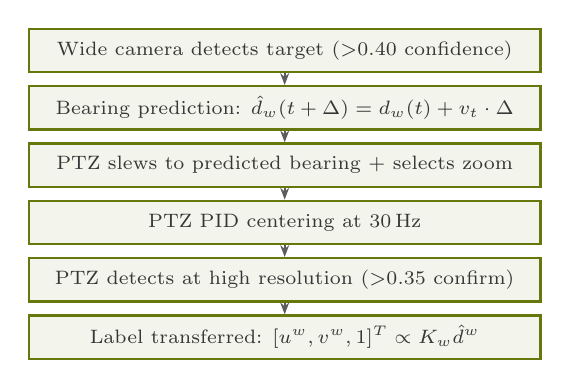
\begin{tikzpicture}[
          pbox/.style={rectangle, draw=Horseshoe, fill=Horseshoe!8, line width=0.8pt,
                        minimum height=0.55cm, minimum width=6.5cm,
                        font=\scriptsize, align=center, text=Black90},
          arr/.style={-{Stealth[length=1.5mm]}, thick, color=Black70},
          node distance=0.15cm
        ]
          \node[pbox] (s1) {Wide camera detects target ($>$0.40 confidence)};
          \node[pbox, below=of s1] (s2) {Bearing prediction: $\hat{d}_w(t+\Delta) = d_w(t) + v_t \cdot \Delta$};
          \node[pbox, below=of s2] (s3) {PTZ slews to predicted bearing + selects zoom};
          \node[pbox, below=of s3] (s4) {PTZ PID centering at 30\,Hz};
          \node[pbox, below=of s4] (s5) {PTZ detects at high resolution ($>$0.35 confirm)};
          \node[pbox, below=of s5] (s6) {Label transferred: $[u^w, v^w, 1]^T \propto K_w \hat{d}^w$};
          \draw[arr] (s1)--(s2); \draw[arr] (s2)--(s3);
          \draw[arr] (s3)--(s4); \draw[arr] (s4)--(s5);
          \draw[arr] (s5)--(s6);
        \end{tikzpicture}
      \end{block}
    \end{column}
    \begin{column}{0.42\textwidth}
      \begin{block}{Quality Gates}
        {\scriptsize
        \begin{itemize}\setlength{\itemsep}{0pt}\setlength{\topsep}{0pt}
          \item PTZ confirm threshold: 0.35
          \item Class agreement required
          \item Motion blur rejection
          \item Exposure validation
          \item Boundary rejection
        \end{itemize}
        }
      \end{block}
      \vspace{0.1em}
      \begin{block}{Five-State Machine}
        \centering
        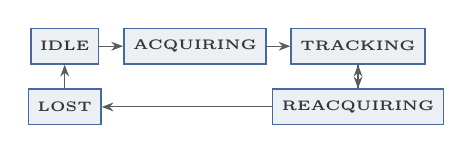
\begin{tikzpicture}[
          sbox/.style={rectangle, draw=Atlantic, fill=Atlantic!10, line width=0.6pt,
                        minimum height=0.45cm, font=\tiny\bfseries, text=Black90},
          arr/.style={-{Stealth[length=1.5mm]}, thin, color=Black70},
          node distance=0.15cm and 0.3cm
        ]
          \node[sbox] (idle) {IDLE};
          \node[sbox, right=of idle] (acq) {ACQUIRING};
          \node[sbox, right=of acq] (trk) {TRACKING};
          \node[sbox, below=0.3cm of trk] (reacq) {REACQUIRING};
          \node[sbox, below=0.3cm of idle] (lost) {LOST};
          \draw[arr] (idle)--(acq);
          \draw[arr] (acq)--(trk);
          \draw[arr] (trk)--(reacq);
          \draw[arr] (reacq)--(trk);
          \draw[arr] (reacq)--(lost);
          \draw[arr] (lost)--(idle);
        \end{tikzpicture}
      \end{block}
    \end{column}
  \end{columns}
\end{frame}

% =============================================================================
% SUMMARY
% =============================================================================
\begin{frame}{Summary}
  \begin{columns}[T]
    \begin{column}{0.55\textwidth}
      \begin{block}{Unified Perception Pipeline}
        \centering
        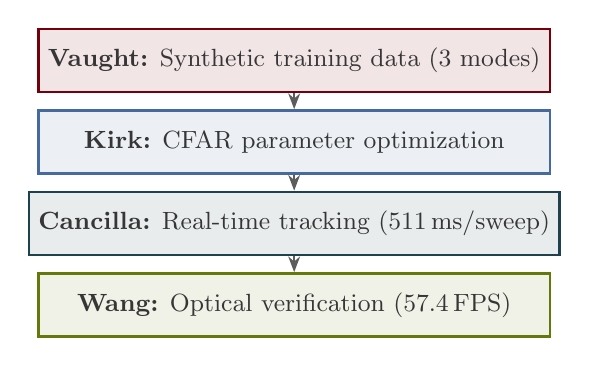
\begin{tikzpicture}[
          arr/.style={-{Stealth[length=2mm]}, thick, color=Black70},
          node distance=0.2cm
        ]
          \node[summbox=Garnet] (s1)
            {\textbf{Vaught:} Synthetic training data (3 modes)};
          \node[summbox=Atlantic, below=of s1] (s2)
            {\textbf{Kirk:} CFAR parameter optimization};
          \node[summbox=Congaree, below=of s2] (s3)
            {\textbf{Cancilla:} Real-time tracking (511\,ms/sweep)};
          \node[summbox=Horseshoe, below=of s3] (s4)
            {\textbf{Wang:} Optical verification (57.4\,FPS)};
          \draw[arr] (s1)--(s2); \draw[arr] (s2)--(s3); \draw[arr] (s3)--(s4);
        \end{tikzpicture}
      \end{block}
    \end{column}
    \begin{column}{0.42\textwidth}
      \begin{block}{Key Takeaways}
        {\scriptsize
        \begin{itemize}\setlength{\itemsep}{0pt}\setlength{\topsep}{0pt}
          \item All COTS sensors, no custom hardware
          \item Edge-deployable on Jetson / RPi5
          \item Real-time performance demonstrated
          \item Open-source tools (CFAR Studio)
          \item Field-validated at 3 SC sites
        \end{itemize}
        }
      \end{block}
      \vspace{0.1em}
      \begin{block}{Future Work}
        {\scriptsize
        \begin{itemize}\setlength{\itemsep}{0pt}\setlength{\topsep}{0pt}
          \item Complete YOLO domain-transfer evaluation
          \item Kalman filtering + MHT for tracking
          \item AIS fusion for ground truth
          \item Multi-PTZ scheduling
          \item Full system integration test
        \end{itemize}
        }
      \end{block}
    \end{column}
  \end{columns}
\end{frame}

% --- Questions ---
\begin{frame}[plain]
  \begin{tikzpicture}[remember picture, overlay]
    \fill[Garnet] (current page.south west) rectangle (current page.north east);
    \node[anchor=center, text=white, font=\Huge\bfseries] at ([yshift=0.8cm]current page.center) {Questions?};
    \node[anchor=center, text=Black30, font=\normalsize] at ([yshift=-0.5cm]current page.center) {%
      J.C.~Vaught \enspace $\cdot$ \enspace N.~Kirk \enspace $\cdot$ \enspace S.~Cancilla \enspace $\cdot$ \enspace J.~Wang%
    };
    \node[anchor=center, text=Black30, font=\small] at ([yshift=-1.3cm]current page.center) {%
      Department of Mechanical Engineering, University of South Carolina%
    };
  \end{tikzpicture}
\end{frame}

\end{document}
